
\documentclass[10pt,a4paper,oneside]{report}
\usepackage[margin=19mm,top=21mm,bottom=22mm]{geometry}
\usepackage{fontspec}
\setmainfont{DejaVu Sans}
\setsansfont{DejaVu Sans}
\setmonofont[Scale=0.82]{DejaVu Sans Mono}
\usepackage{microtype}
\usepackage[dvipsnames]{xcolor}
\usepackage{amsmath,amssymb,booktabs,longtable,tabularx,array}
\usepackage{enumitem}
\usepackage{graphicx}
\usepackage{tikz}
\usetikzlibrary{arrows.meta,positioning,fit,calc}
\usepackage[most]{tcolorbox}
\usepackage{fancyhdr}
\usepackage{titlesec}
\usepackage{hyperref}
\hypersetup{colorlinks=true,linkcolor=NavyBlue,urlcolor=RoyalBlue,pdftitle={Eleven Open-Source Music Players - Architecture, UI/UX and Implementation Blueprints},pdfauthor={Technical Research Report}}
\definecolor{ink}{HTML}{112033}
\definecolor{muted}{HTML}{4D6175}
\definecolor{navy}{HTML}{143550}
\definecolor{teal}{HTML}{087F8C}
\definecolor{light}{HTML}{EDF5F8}
\definecolor{line}{HTML}{D5E1E7}
\color{ink}
\titleformat{\chapter}[display]{\normalfont\Huge\bfseries\color{navy}}{\small\color{teal}\MakeUppercase{Project \thechapter}}{4pt}{}
\titlespacing*{\chapter}{0pt}{-8pt}{14pt}
\titleformat{\section}{\large\bfseries\color{navy}}{\thesection}{8pt}{}
\titlespacing*{\section}{0pt}{12pt}{5pt}
\titleformat{\subsection}{\normalsize\bfseries\color{teal}}{\thesubsection}{6pt}{}
\titlespacing*{\subsection}{0pt}{8pt}{3pt}
\setlength{\parindent}{0pt}
\setlength{\parskip}{4pt}
\setlength{\emergencystretch}{4em}
\pagestyle{fancy}
\fancyhf{}
\fancyhead[L]{\scriptsize\color{muted} MUSIC PLAYER ARCHITECTURE + UX ATLAS}
\fancyhead[R]{\scriptsize\color{muted} RESEARCH SNAPSHOT: 14 OCT 2026}
\fancyfoot[L]{\scriptsize\color{muted} Verified evidence / proposed implementation separated}
\fancyfoot[R]{\scriptsize\color{navy}\thepage}
\renewcommand{\headrulewidth}{0.3pt}
\renewcommand{\footrulewidth}{0pt}
\newtcolorbox{evidencebox}{colback=light,colframe=line,boxrule=0.4pt,arc=1.5mm,left=3mm,right=3mm,top=2mm,bottom=2mm}
\newcommand{\tagverified}{\textbf{[V] Verified from public project documentation / repository layout.}}
\newcommand{\tagproposal}{\textbf{[P] Proposed blueprint; not an assertion of existing source.}}
\newcommand{\tagboundary}{\textbf{[B] Evidence boundary or known project constraint.}}
\newcommand{\sourceurl}[1]{\href{#1}{\texttt{\nolinkurl{#1}}}}
\begin{document}
\begin{titlepage}
\pagecolor{navy}\color{white}
\vspace*{25mm}
{\Large TECHNICAL RESEARCH SERIES}\par\vspace{10mm}
{\fontsize{30}{36}\selectfont\bfseries Eleven Open-Source\\Music Players}\par\vspace{7mm}
{\fontsize{20}{26}\selectfont Architecture, UI/UX and Implementation Blueprints}\par\vspace{12mm}
{\color{white!80}\large 11 profiles | LaTeX diagrams | Visual UI concepts |\par
Playback paths | UX journeys | Accessibility | Build plans}\par
\vfill
{\large Evidence reviewed: 14 October 2026}\par\vspace{4mm}
{\small 11 independently documented applications. Reusable reference designs, not reverse-engineered internal specifications.}\par\vspace{15mm}
\end{titlepage}
\pagecolor{white}\color{ink}
\pagenumbering{roman}
\chapter*{How to read this report}
\addcontentsline{toc}{chapter}{How to read this report}
This is a combined architecture and UI/UX atlas for the 11 projects selected in the preceding comparison: Feishin, Tauon, Koel, Swing Music, Museeks, Strawberry, Finamp, Gramophone, Auxio, Retro Music Player, and Music Assistant.
\begin{evidencebox}
\tagverified{} Explicitly supported by the public GitHub repository, its README, build metadata, its visible top-level structure, or project technical documentation.\\[3pt]
\tagproposal{} An engineering design suitable for building a comparable application; names, schemas, algorithms and contracts under this label must \emph{not} be attributed to the project's actual source.\\[3pt]
\tagboundary{} A dependency, license limit, confidence limit or known missing verification.
\end{evidencebox}
\textbf{Research scope.} The evidence is a dated, public documentation review rather than a local clone, complete static-analysis pass, executable test run or reproducible binary audit. Directory anchors identify where to begin source inspection; only explicitly cited files and stated top-level roots were established. No undocumented private APIs, precise class diagrams or audio-measurement results are invented. GitHub default branches are mutable; confirm the current revision and dependencies before implementation. Audio capability descriptions are not DAC measurements.

\textbf{License notice.} License labels summarize repository-level statements, not legal advice. Inspect file-level headers, third-party components, premium modules, patents, artwork, trademarks and app-store policy before redistribution. Browser FLAC decoding, lossless transport and bit-perfect hardware output are distinct claims.

\setcounter{tocdepth}{0}
\tableofcontents
\clearpage
\pagenumbering{arabic}
\chapter*{Cross-system architectural map}
\addcontentsline{toc}{chapter}{Cross-system architectural map}
\begin{longtable}{@{}p{34mm}p{32mm}p{43mm}p{45mm}@{}}
\toprule
Project & Deployment shape & Principal media source & Primary differentiation\\\midrule\endhead
Feishin & Desktop + web & Jellyfin / OpenSubsonic & Dual MPV/web playback\\
Tauon & Desktop & Local / optional server & Native Phazor, gapless\\
Koel & Full-stack web & Self-hosted folders & Scanner + Vue/Laravel\\
Swing Music & Self-hosted server & Local music volumes & Personalization + polished UI\\
Museeks & Tauri desktop & Local files & Lean MIT product base\\
Strawberry & Qt desktop & Local / select streams & Audiophile metadata/output\\
Finamp & Flutter clients & Jellyfin & Offline sync + gapless\\
Gramophone & Android native & MediaStore & Media3 + synchronized lyrics\\
Auxio & Android native & MediaStore + tags & Privacy + advanced metadata\\
Retro Music & Android native & MediaStore & Themeable player presentation\\
Music Assistant & Server + Vue PWA & Provider plugins & Multi-device orchestration\\
\bottomrule
\end{longtable}
\section*{Evidence fidelity rules}
\begin{itemize}[leftmargin=*]
\item \textbf{Runtime architecture:} distinguish a player that owns local files from a thin client that consumes a separate server.
\item \textbf{Data flow:} catalog metadata (small HTTP/database records) is not interchangeable with audio payload (file, URL, PCM or HTTP stream).
\item \textbf{Licensing:} an open repository does not automatically open source premium compiled modules or separate server components.
\item \textbf{Audio quality:} lossless decoding does not guarantee an unchanged output signal. EQ, normalization, DSP, transcoding, resampling and OS mixing can modify samples.
\end{itemize}
\clearpage
\chapter{Feishin}
{\large\color{muted}Electron and web client for external music servers}\par
\begin{evidencebox}\small\textbf{Repository:} \sourceurl{https://github.com/jeffvli/feishin}\\\textbf{Reference branch:} development\qquad \textbf{License:} GPL-3.0\\\textbf{Primary stack:} TypeScript; React-oriented web renderer; Electron desktop shell; Vite/pnpm; MPV or browser playback.\end{evidencebox}
\section{Observed system architecture [V]}
\begin{itemize}[leftmargin=*,itemsep=2pt,topsep=3pt]
\item The same project builds an Electron desktop application and a standalone web renderer; web playback excludes desktop-only MPV.
\item It connects to Jellyfin, Navidrome and compatible OpenSubsonic servers; server ownership and indexing are external.
\item Documented features include smart playlists (Navidrome), scrobbling and synchronized/unsynchronized lyrics.
\end{itemize}
\textbf{Visible source anchors [V].} src/, docs/, electron.vite.config.ts, web.vite.config.ts, remote.vite.config.ts, package.json, Dockerfile.\par
\begin{evidencebox}\tagboundary{} The repository description establishes the external-server and dual-backend shape; exact internal hooks, state store, transport methods, and persistence schema were not code-audited.\end{evidencebox}
\section{Functional block blueprint [P]}
\begin{center}
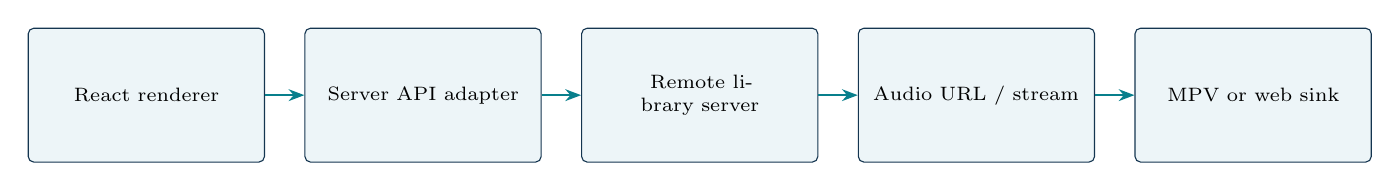
\begin{tikzpicture}[>=Stealth, node distance=1.4mm, every node/.style={font=\scriptsize,align=center}]
\node[draw=navy,rounded corners=2pt,fill=light,text width=26mm,minimum height=17mm,inner sep=2mm] (n0) {React renderer};
\node[draw=navy,rounded corners=2pt,fill=light,text width=26mm,minimum height=17mm,inner sep=2mm,right=5mm of n0] (n1) {Server API adapter};
\draw[-{Stealth[length=2mm]},thick,color=teal] (n0.east) -- (n1.west);
\node[draw=navy,rounded corners=2pt,fill=light,text width=26mm,minimum height=17mm,inner sep=2mm,right=5mm of n1] (n2) {Remote library server};
\draw[-{Stealth[length=2mm]},thick,color=teal] (n1.east) -- (n2.west);
\node[draw=navy,rounded corners=2pt,fill=light,text width=26mm,minimum height=17mm,inner sep=2mm,right=5mm of n2] (n3) {Audio URL / stream};
\draw[-{Stealth[length=2mm]},thick,color=teal] (n2.east) -- (n3.west);
\node[draw=navy,rounded corners=2pt,fill=light,text width=26mm,minimum height=17mm,inner sep=2mm,right=5mm of n3] (n4) {MPV or web sink};
\draw[-{Stealth[length=2mm]},thick,color=teal] (n3.east) -- (n4.west);
\end{tikzpicture}
\end{center}
\small\textit{Figure 1: Conceptual runtime path for a comparable implementation. This is not a traced source-code call graph.}\normalsize\par
\section{End-to-end user-to-speaker flow}
\begin{enumerate}[leftmargin=*,itemsep=2pt,topsep=2pt]
\item User selects an album or track in the renderer.
\item A normalized server adapter fetches metadata and resolves a streamable media item.
\item Queue controller assigns ordered entries; desktop chooses MPV or browser backend.
\item The selected engine requests media from the user-configured server.
\item Playback state, lyrics timing and eligible scrobble events update the UI/server.
\end{enumerate}
\section{Data contract [P]}
\begin{evidencebox}\small\textbf{Candidate conceptual entities (not copied database classes):}\par
\begin{itemize}[leftmargin=*,itemsep=1pt,topsep=2pt]
\item \texttt{ServerProfile(id, type, base\_url, auth\_ref)}
\item \texttt{MediaItem(id, server\_id, artist\_id, album\_id, codec)}
\item \texttt{QueueEntry(queue\_id, position, media\_id)}
\item \texttt{PlaybackState(position\_ms, repeat, shuffle)}
\item \texttt{LyricsLine(time\_ms, text)}
\end{itemize}\end{evidencebox}
\section{Implementation blueprint [P]}
\begin{itemize}[leftmargin=*,itemsep=2pt,topsep=3pt]
\item Keep server-specific adapters behind a LibraryGateway with getArtist, getAlbum, search, and resolveStream methods.
\item Specify a single PlaybackPort contract for load, play, pause, seek, volume and state events; provide separate MPV and HTMLMedia implementations.
\item Model capabilities per server and per player (smart playlists, scrobbling, lyrics, transcoding, gapless) rather than hiding unsupported features.
\item Place access tokens in OS credential storage for desktop; use a secure session strategy for web; never embed remote-server secrets in public bundles.
\item Create a shared queue/now-playing state machine, with explicit transitions IDLE, LOADING, PLAYING, PAUSED, ERROR.
\item Ship separate Electron, web and container builds; exercise each path in CI.
\end{itemize}
\subsection*{Engineering equation}
\begin{equation*}\mathrm{CanPlay}(m,p,s)=\mathrm{CodecOK}(m,p)\land\mathrm{AuthOK}(s)\land\mathrm{URLResolved}(m,s)\end{equation*}
A stream is playable only if the backend supports the codec and the remote server authorizes and resolves it.\par
\section{Validation and operational guardrails}
\textbf{Acceptance-test plan [P].}\par
\begin{itemize}[leftmargin=*,itemsep=2pt,topsep=3pt]
\item Integration tests against at least one Jellyfin and one OpenSubsonic-compatible server.
\item Desktop MPV versus web media-element parity matrix: seek, end-of-track, buffering, lyrics and scrobble thresholds.
\item Failure injection for stale credentials, expired stream URLs and network disconnects.
\end{itemize}
\textbf{Constraints and risks [B].}\par
\begin{itemize}[leftmargin=*,itemsep=2pt,topsep=3pt]
\item Not a standalone scanner or library server; installation alone does not supply music.
\item Browser playback is governed by browser codecs and media-output limitations.
\item GPL obligations apply when redistributing derivatives.
\end{itemize}
\section*{Primary evidence and source entry points}
\begin{itemize}[leftmargin=*,itemsep=1pt,topsep=1pt]
\item \sourceurl{https://github.com/jeffvli/feishin}
\item \sourceurl{https://github.com/jeffvli/feishin/blob/development/README.md}
\end{itemize}
\clearpage
\section{UI/UX architecture and annotated screen concept}
\begin{evidencebox}\small\tagverified{} The public project documents desktop MPV and web playback, synchronized/unsynchronized lyrics, and Navidrome smart playlists. Its README includes interface screenshots, but the proposed screen below is not a captured current release.\\[2pt]\textbf{UX evidence link:} \sourceurl{https://github.com/jeffvli/feishin/blob/development/README.md}\\[2pt]\tagproposal{} The image, colors, exact screen compositions, flows, and acceptance criteria below are authored design recommendations, not release screenshots or audited internal UI components.\end{evidencebox}
\begin{center}
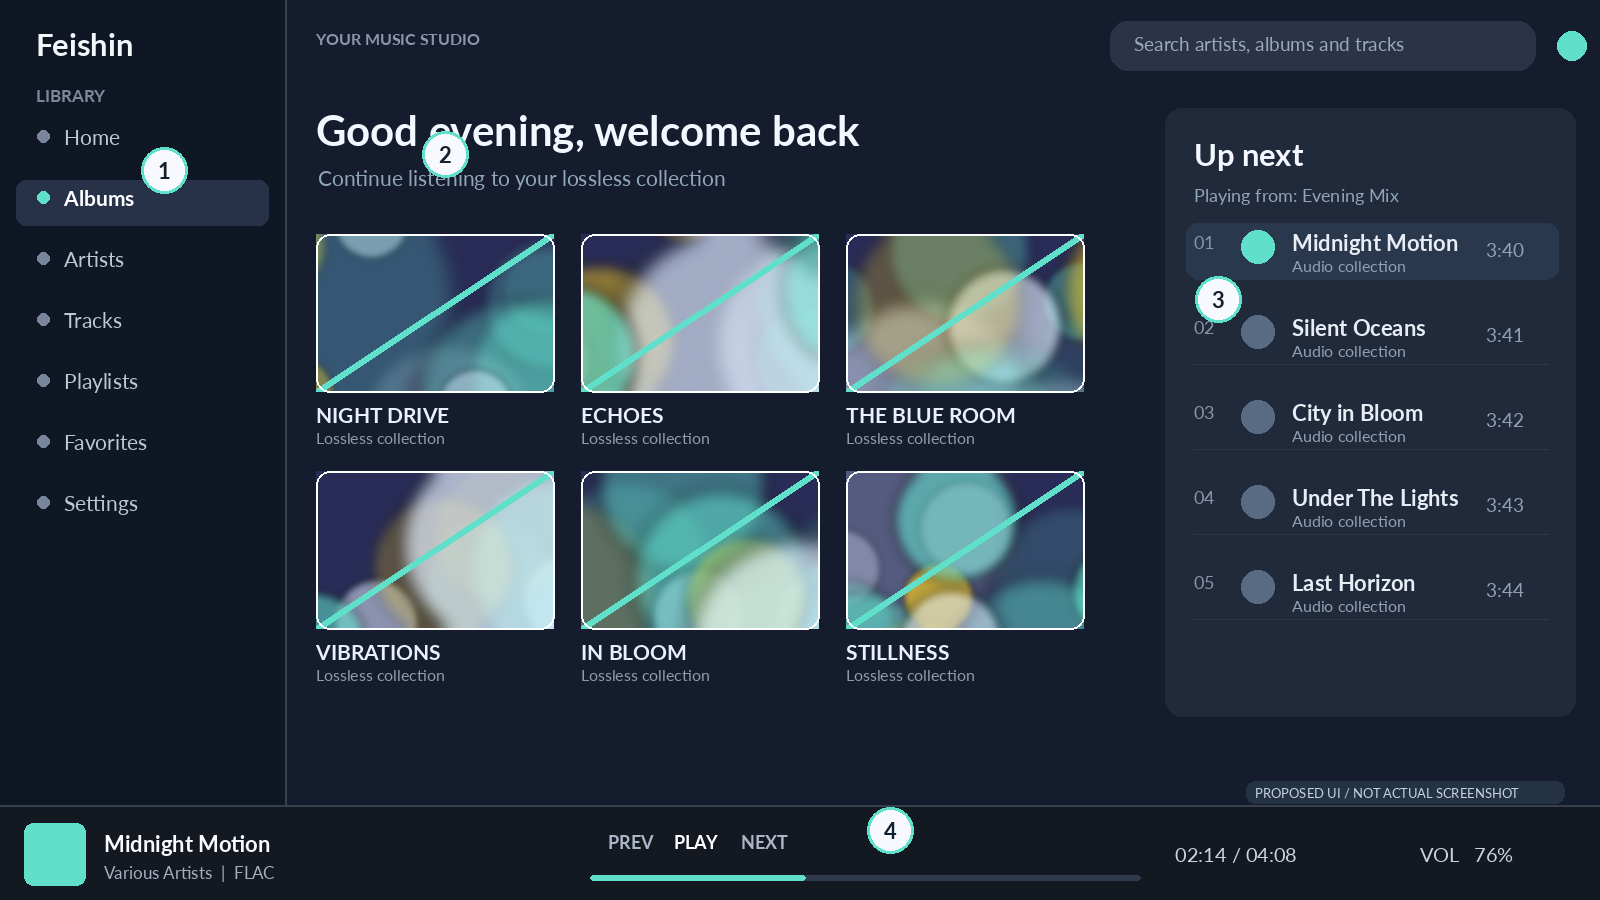
\includegraphics[width=\linewidth,height=93mm,keepaspectratio]{Music_Player_UIUX_Assets/feishin_concept.png}
\end{center}
{\small\color{muted}\textit{Annotated concept:} Dense, art-forward browsing with persistent queue and a stable playback bar. Surface server identity and the chosen playback backend. \textbf{Intended platform:} Desktop + responsive web. The visual uses invented album names and placeholder artwork.\par}
\subsection*{Proposed visual design system}
\begin{tabularx}{\linewidth}{@{}p{24mm}X@{}}
\textbf{Palette} & \colorbox[HTML]{141C2D}{\rule{6mm}{3mm}}\, Base 141C2D \quad \colorbox[HTML]{60DFCB}{\rule{6mm}{3mm}}\, Accent 60DFCB \\
\textbf{Typography} & Body 14--16 px; labels 12--13 px; primary screen heading 26--34 px; numeric audio data set in tabular figures.\\
\textbf{Spacing} & 4/8 px grid; 8--16 px card radius; align cover art to text blocks; 44 px touch-target minimum where relevant.\\
\textbf{Contrast} & Target WCAG AA text contrast, 4.5:1 for normal text and 3:1 for large text; verify final palette in both light/dark states.\\
\end{tabularx}
\subsection*{Annotated interface anatomy}
\begin{tabularx}{\linewidth}{@{}p{12mm}X@{}}\toprule Mark & Proposed region and responsibilities\\\midrule
\textbf{1} & Library and server navigation with explicit connected-source identity\\
\textbf{2} & Album and playlist cards with keyboard-safe action targets\\
\textbf{3} & Queue/lyrics inspector with selection and active-track highlighting\\
\textbf{4} & Pinned transport: time, selected backend and error feedback\\
\bottomrule\end{tabularx}
\clearpage
\section{UX functional specification [P]}
\subsection*{Information architecture and screens}
\begin{tabularx}{\linewidth}{@{}p{34mm}X@{}}\toprule Screen / route & Core content and controls\\\midrule
Connect server & Server type, URL, credentials, test connection and actionable failures\\
Home / Library & Albums, artists, saved mixes, recent history and search\\
Album detail & Artwork, track list, batch add, play/shuffle and provenance\\
Now playing + lyrics & Fullscreen art, line-synced lyrics, timing offset and queue drawer\\
Settings / audio & Server, MPV-versus-web backend, output behavior and scrobbling\\
\bottomrule\end{tabularx}
\subsection*{Navigation model}
Left navigation on desktop; compact navigation and bottom player on narrow web layouts. Queue/lyrics as a right-side panel or full-screen mobile sheet.\par
\subsection*{Critical user journeys}
\begin{enumerate}[leftmargin=*,itemsep=3pt,topsep=2pt]
\item \textbf{First-run connect.} Open onboarding; validate server address; sign in; load library; land on Home.
\item \textbf{Play from search.} Focus global search; inspect result; add or replace queue; begin playback; show source server.
\item \textbf{Lyrics and queue.} Open now-playing; choose synced or plain lyrics; shift queue entry; preserve current timestamp.
\end{enumerate}
\subsection*{Interaction, feedback and edge states}
Space toggles playback when no text field is active; keyboard reorder controls; hover and focus previews; selected queue row follows playhead.\par
\begin{tabularx}{\linewidth}{@{}p{39mm}X@{}}\toprule State / trigger & Expected UX behavior\\\midrule
Server unavailable & Retain cached catalog visually; mark offline; offer Retry and Change server.\\
Playback unsupported & Show backend-specific error and offer compatible engine, not silent substitution.\\
Lyrics missing & Display a non-blocking no-lyrics state while audio remains controllable.\\
\bottomrule\end{tabularx}
\subsection*{Implementation and QA contract}
\begin{itemize}[leftmargin=*,itemsep=2pt,topsep=2pt]
\item \textbf{Single source of truth.} Playback, queue and current destination/device belong to the application state model, not duplicated per view.
\item \textbf{Accessibility.} Keyboard navigation, screen-reader labels, visible focus, user-controlled lyric scrolling, reduced motion and non-color-only states.
\item \textbf{Responsive behavior.} Preserve transport when resizing; test narrow, zoomed and high-font settings; use alternative to drag-only controls.
\item \textbf{Instrumentation.} time-to-first-play; server-login completion; search-to-play; lyrics load; queue reorder errors.
\item \textbf{Boundary.} Do not label desktop-only MPV sound modes as available in a browser. Streaming quality depends on the remote server and settings.
\end{itemize}
\vspace{2mm}\begin{evidencebox}\small\textbf{Prototype acceptance:} Primary play and pause remain available through every screen; the queue and playback position survive navigation; every error has recovery text; every advertised fidelity setting accurately reflects the active engine/device. Design specifications are recommendations and require product usability testing.\end{evidencebox}
\clearpage
\chapter{Tauon}
{\large\color{muted}Desktop-first library manager with native playback engine}\par
\begin{evidencebox}\small\textbf{Repository:} \sourceurl{https://github.com/Taiko2k/Tauon}\\\textbf{Reference branch:} master\qquad \textbf{License:} GPL-3.0\\\textbf{Primary stack:} Python application; C-based Phazor native playback extension; local audio library; optional Plex/Jellyfin/Airsonic integrations.\end{evidencebox}
\section{Observed system architecture [V]}
\begin{itemize}[leftmargin=*,itemsep=2pt,topsep=3pt]
\item Modern source packaging defines native extensions named phazor and phazor-pw, including decoding and resampling dependencies.
\item The application documents FLAC, tracker codecs, gapless playback, CUE sheets, visualizers, themed UI and optional network sources.
\item The changelog reports removal of its GStreamer backend; old setup pages mentioning GStreamer are not current implementation evidence.
\end{itemize}
\textbf{Visible source anchors [V].} src/, src/phazor/, src/tauon/, src/tauon/t\_modules/, pyproject.toml, packaging/, tools/.\par
\begin{evidencebox}\tagboundary{} The C-extension presence and Python package layout are source-backed; precise DSP order, audio-thread implementation and library schema need full source inspection.\end{evidencebox}
\section{Functional block blueprint [P]}
\begin{center}
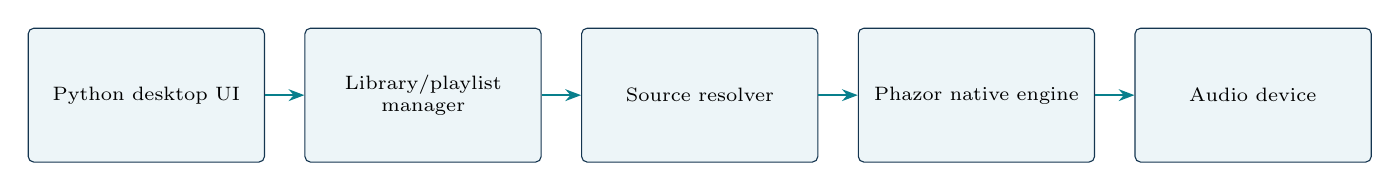
\begin{tikzpicture}[>=Stealth, node distance=1.4mm, every node/.style={font=\scriptsize,align=center}]
\node[draw=navy,rounded corners=2pt,fill=light,text width=26mm,minimum height=17mm,inner sep=2mm] (n0) {Python desktop UI};
\node[draw=navy,rounded corners=2pt,fill=light,text width=26mm,minimum height=17mm,inner sep=2mm,right=5mm of n0] (n1) {Library/playlist manager};
\draw[-{Stealth[length=2mm]},thick,color=teal] (n0.east) -- (n1.west);
\node[draw=navy,rounded corners=2pt,fill=light,text width=26mm,minimum height=17mm,inner sep=2mm,right=5mm of n1] (n2) {Source resolver};
\draw[-{Stealth[length=2mm]},thick,color=teal] (n1.east) -- (n2.west);
\node[draw=navy,rounded corners=2pt,fill=light,text width=26mm,minimum height=17mm,inner sep=2mm,right=5mm of n2] (n3) {Phazor native engine};
\draw[-{Stealth[length=2mm]},thick,color=teal] (n2.east) -- (n3.west);
\node[draw=navy,rounded corners=2pt,fill=light,text width=26mm,minimum height=17mm,inner sep=2mm,right=5mm of n3] (n4) {Audio device};
\draw[-{Stealth[length=2mm]},thick,color=teal] (n3.east) -- (n4.west);
\end{tikzpicture}
\end{center}
\small\textit{Figure 2: Conceptual runtime path for a comparable implementation. This is not a traced source-code call graph.}\normalsize\par
\section{End-to-end user-to-speaker flow}
\begin{enumerate}[leftmargin=*,itemsep=2pt,topsep=2pt]
\item User adds local music folders or a supported remote source.
\item Scanner extracts tags and cover information; playlist and folder indexes update.
\item Queue resolves the next local path, CUE segment, or remote stream.
\item Phazor decodes frames and delivers them to the configured device/output.
\item Playback progress and visualizer measurements update desktop components.
\end{enumerate}
\section{Data contract [P]}
\begin{evidencebox}\small\textbf{Candidate conceptual entities (not copied database classes):}\par
\begin{itemize}[leftmargin=*,itemsep=1pt,topsep=2pt]
\item \texttt{Track(path, codec, tags, replay\_gain)}
\item \texttt{Album(artist, title, edition, artwork)}
\item \texttt{PlaylistEntry(playlist\_id, order, track\_id)}
\item \texttt{OutputConfig(device\_id, sample\_rate, resample\_mode)}
\item \texttt{CueSegment(file\_id, start\_ms, end\_ms)}
\end{itemize}\end{evidencebox}
\section{Implementation blueprint [P]}
\begin{itemize}[leftmargin=*,itemsep=2pt,topsep=3pt]
\item Make a Python domain layer independent of widgets: scanner, library index, playlist, metadata and artwork.
\item Expose a narrow native audio FFI with create, load, seek, set-output, start, stop, and callback methods.
\item Keep decoding, resampling and audio device writing off the UI thread; use bounded buffers.
\item Treat CUE entries as views over a shared audio file; do not duplicate data on disk.
\item Create explicit per-backend device and sample-rate capabilities; surface resampling status to audiophile users.
\item Place network-source connectors behind an optional provider interface and keep their auth separate from local library indexing.
\end{itemize}
\subsection*{Engineering equation}
\begin{equation*}T_{\mathrm{buffer}}=\frac{N_{\mathrm{frames}}}{f_s},\qquad B_{\mathrm{PCM}}=N_{\mathrm{frames}}\,c\,b/8\end{equation*}
Buffer duration and PCM buffer bytes depend on the frame count, output sample rate, channel count c and sample width b.\par
\section{Validation and operational guardrails}
\textbf{Acceptance-test plan [P].}\par
\begin{itemize}[leftmargin=*,itemsep=2pt,topsep=3pt]
\item Deterministic gapless test between adjacent lossless files and CUE segments.
\item Output-device switching, decoder crash isolation and corrupted-tag handling.
\item Resampling and crossfade-off listening checks; no unverified bit-perfect promise.
\end{itemize}
\textbf{Constraints and risks [B].}\par
\begin{itemize}[leftmargin=*,itemsep=2pt,topsep=3pt]
\item Native extensions complicate platform packaging and codec licensing diligence.
\item Older Tauon pages refer to GStreamer although current changelog says it was removed.
\item GPL governs redistribution of modified binaries.
\end{itemize}
\section*{Primary evidence and source entry points}
\begin{itemize}[leftmargin=*,itemsep=1pt,topsep=1pt]
\item \sourceurl{https://github.com/Taiko2k/Tauon}
\item \sourceurl{https://github.com/Taiko2k/Tauon/blob/master/pyproject.toml}
\item \sourceurl{https://github.com/Taiko2k/Tauon/blob/master/CHANGELOG.md}
\end{itemize}
\clearpage
\section{UI/UX architecture and annotated screen concept}
\begin{evidencebox}\small\tagverified{} The repository documents adaptive theming, gapless playback, CUE handling, widget customization and visualizations. The official manual documents lyrics in a side panel and a Showcase + Lyrics view.\\[2pt]\textbf{UX evidence link:} \sourceurl{https://tauonmusicbox.rocks/manual/lyrics}\\[2pt]\tagproposal{} The image, colors, exact screen compositions, flows, and acceptance criteria below are authored design recommendations, not release screenshots or audited internal UI components.\end{evidencebox}
\begin{center}
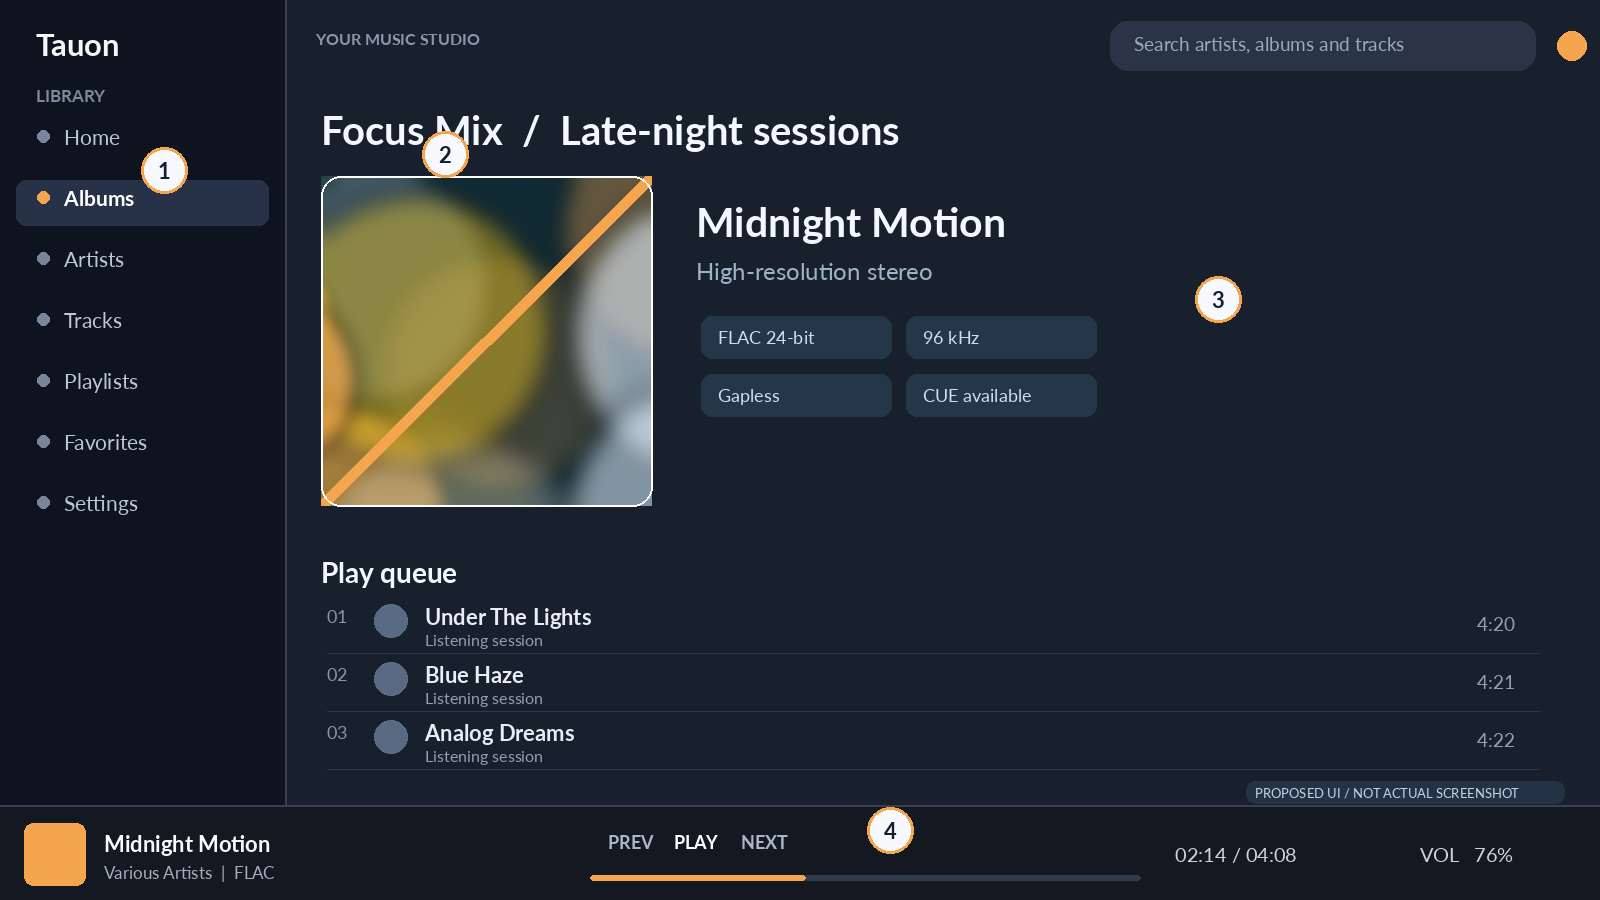
\includegraphics[width=\linewidth,height=93mm,keepaspectratio]{Music_Player_UIUX_Assets/tauon_concept.png}
\end{center}
{\small\color{muted}\textit{Annotated concept:} Album-art-first player emphasizing collection immersion and responsive visual feedback without obscuring advanced audio metadata. \textbf{Intended platform:} Desktop. The visual uses invented album names and placeholder artwork.\par}
\subsection*{Proposed visual design system}
\begin{tabularx}{\linewidth}{@{}p{24mm}X@{}}
\textbf{Palette} & \colorbox[HTML]{17202C}{\rule{6mm}{3mm}}\, Base 17202C \quad \colorbox[HTML]{F4A54E}{\rule{6mm}{3mm}}\, Accent F4A54E \\
\textbf{Typography} & Body 14--16 px; labels 12--13 px; primary screen heading 26--34 px; numeric audio data set in tabular figures.\\
\textbf{Spacing} & 4/8 px grid; 8--16 px card radius; align cover art to text blocks; 44 px touch-target minimum where relevant.\\
\textbf{Contrast} & Target WCAG AA text contrast, 4.5:1 for normal text and 3:1 for large text; verify final palette in both light/dark states.\\
\end{tabularx}
\subsection*{Annotated interface anatomy}
\begin{tabularx}{\linewidth}{@{}p{12mm}X@{}}\toprule Mark & Proposed region and responsibilities\\\midrule
\textbf{1} & Collection tree and saved-queue navigation\\
\textbf{2} & Artwork-focused active session and album metadata\\
\textbf{3} & Audio format and CUE cues: surfaced, not hidden in settings\\
\textbf{4} & Transport/status row, including gapless and output notices\\
\bottomrule\end{tabularx}
\clearpage
\section{UX functional specification [P]}
\subsection*{Information architecture and screens}
\begin{tabularx}{\linewidth}{@{}p{34mm}X@{}}\toprule Screen / route & Core content and controls\\\midrule
Collection grid & Folder/playlist browsing, sort and filters\\
Queue and transport & Drag/drop ordering, next-up items and playback controls\\
Showcase + lyrics & Rich visual scene, lyrics and synchronized line highlight\\
Audio information & File format, rate, cue segments, output and visualizer status\\
Preferences & Widget layout, theme, library sources and remote-server configuration\\
\bottomrule\end{tabularx}
\subsection*{Navigation model}
Persistent compact collection/playlist rail; main context-sensitive canvas; optional lyric/widget dock; bottom player continuity.\par
\subsection*{Critical user journeys}
\begin{enumerate}[leftmargin=*,itemsep=3pt,topsep=2pt]
\item \textbf{Import music.} Pick music folders; show indexing progress; review duplicates; open collection.
\item \textbf{Enter lyric showcase.} Start playback; open Showcase + Lyrics; switch views; keep keyboard transport.
\item \textbf{Cue-aware playback.} Open an indexed disc; choose cue segment; play; expose chapter boundary.
\end{enumerate}
\subsection*{Interaction, feedback and edge states}
Double-click track to replace queue; drag playlist order; keyboard seek and volume; animation pauses under reduced-motion preference.\par
\begin{tabularx}{\linewidth}{@{}p{39mm}X@{}}\toprule State / trigger & Expected UX behavior\\\midrule
Artwork missing & Render branded color placeholder; retain album title/artist hierarchy.\\
Index in progress & Partial results remain interactive; progress is dismissible and revisitable.\\
No synchronized lyrics & Present plain text or retrieval/edit affordance without a blocking dialog.\\
\bottomrule\end{tabularx}
\subsection*{Implementation and QA contract}
\begin{itemize}[leftmargin=*,itemsep=2pt,topsep=2pt]
\item \textbf{Single source of truth.} Playback, queue and current destination/device belong to the application state model, not duplicated per view.
\item \textbf{Accessibility.} Keyboard navigation, screen-reader labels, visible focus, user-controlled lyric scrolling, reduced motion and non-color-only states.
\item \textbf{Responsive behavior.} Preserve transport when resizing; test narrow, zoomed and high-font settings; use alternative to drag-only controls.
\item \textbf{Instrumentation.} library-scan completion; visualizer frame consistency; queue edit success; gapless boundary UX.
\item \textbf{Boundary.} Visualizer animation and metadata may reflect decoded audio, not an audited bit-perfect output path.
\end{itemize}
\vspace{2mm}\begin{evidencebox}\small\textbf{Prototype acceptance:} Primary play and pause remain available through every screen; the queue and playback position survive navigation; every error has recovery text; every advertised fidelity setting accurately reflects the active engine/device. Design specifications are recommendations and require product usability testing.\end{evidencebox}
\clearpage
\chapter{Koel}
{\large\color{muted}Full-stack personal streaming service and browser player}\par
\begin{evidencebox}\small\textbf{Repository:} \sourceurl{https://github.com/koel/koel}\\\textbf{Reference branch:} master\qquad \textbf{License:} MIT (open core); Koel Plus is separate\\\textbf{Primary stack:} Laravel/PHP server; Vue browser UI; Vite; relational data and filesystem-backed personal music library.\end{evidencebox}
\section{Observed system architecture [V]}
\begin{itemize}[leftmargin=*,itemsep=2pt,topsep=3pt]
\item Official description explicitly identifies Laravel and Vue and a scanner that exposes personal media through a browser.
\item Repository structure separates Laravel services, routes, database migrations, public assets and Vue resources.
\item Playlists, smart playlists, scrobbling, podcasts, radio and integrations are described; multi-user, SSO and white-label are Koel Plus features.
\end{itemize}
\textbf{Visible source anchors [V].} app/, routes/, database/, resources/, config/, storage/, api-docs/, tests/, composer.json, package.json.\par
\begin{evidencebox}\tagboundary{} The domain entities below are implementation blueprint entities, not a verbatim transcription of database migration names or public HTTP endpoints.\end{evidencebox}
\section{Functional block blueprint [P]}
\begin{center}
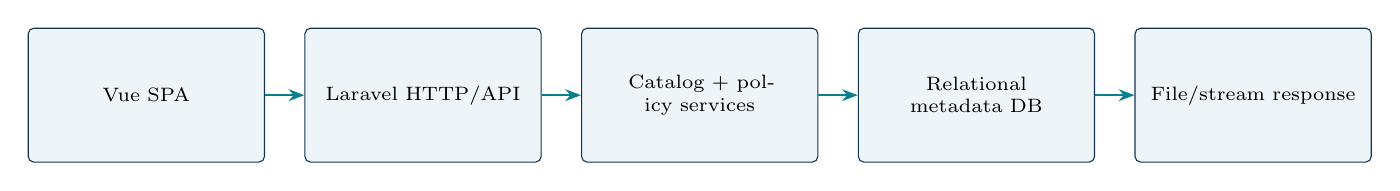
\begin{tikzpicture}[>=Stealth, node distance=1.4mm, every node/.style={font=\scriptsize,align=center}]
\node[draw=navy,rounded corners=2pt,fill=light,text width=26mm,minimum height=17mm,inner sep=2mm] (n0) {Vue SPA};
\node[draw=navy,rounded corners=2pt,fill=light,text width=26mm,minimum height=17mm,inner sep=2mm,right=5mm of n0] (n1) {Laravel HTTP/API};
\draw[-{Stealth[length=2mm]},thick,color=teal] (n0.east) -- (n1.west);
\node[draw=navy,rounded corners=2pt,fill=light,text width=26mm,minimum height=17mm,inner sep=2mm,right=5mm of n1] (n2) {Catalog + policy services};
\draw[-{Stealth[length=2mm]},thick,color=teal] (n1.east) -- (n2.west);
\node[draw=navy,rounded corners=2pt,fill=light,text width=26mm,minimum height=17mm,inner sep=2mm,right=5mm of n2] (n3) {Relational metadata DB};
\draw[-{Stealth[length=2mm]},thick,color=teal] (n2.east) -- (n3.west);
\node[draw=navy,rounded corners=2pt,fill=light,text width=26mm,minimum height=17mm,inner sep=2mm,right=5mm of n3] (n4) {File/stream response};
\draw[-{Stealth[length=2mm]},thick,color=teal] (n3.east) -- (n4.west);
\end{tikzpicture}
\end{center}
\small\textit{Figure 3: Conceptual runtime path for a comparable implementation. This is not a traced source-code call graph.}\normalsize\par
\section{End-to-end user-to-speaker flow}
\begin{enumerate}[leftmargin=*,itemsep=2pt,topsep=2pt]
\item Admin configures folders and runs or schedules media scanning.
\item Scanner reads file metadata, normalizes entities and persists a catalog index.
\item Vue requests search, playlists, artwork and track metadata via server endpoints.
\item Authorized playback request resolves protected local content and returns a media response.
\item Client reports listened progress and relevant integrations receive scrobbles.
\end{enumerate}
\section{Data contract [P]}
\begin{evidencebox}\small\textbf{Candidate conceptual entities (not copied database classes):}\par
\begin{itemize}[leftmargin=*,itemsep=1pt,topsep=2pt]
\item \texttt{User(id, auth\_policy)}
\item \texttt{Track(id, path, duration, audio\_format)}
\item \texttt{Artist(id, name)}
\item \texttt{Album(id, artist\_id, artwork\_path)}
\item \texttt{Playlist(id, owner\_id); PlaylistTrack(order)}
\item \texttt{ListeningEvent(user\_id, track\_id, offset\_ms)}
\end{itemize}\end{evidencebox}
\section{Implementation blueprint [P]}
\begin{itemize}[leftmargin=*,itemsep=2pt,topsep=3pt]
\item Separate media ingestion from playback: scanner job, tag normalizer, cover extractor, catalog updater.
\item Implement an HTTP boundary with request validation, authorization, pagination and rate limiting.
\item Index track path, artist, album, duration, codec and stable fingerprint; preserve manual metadata overrides.
\item Use range-aware media delivery for seekable HTTP playback and an optional transcoding worker.
\item Keep a frontend domain store for browse, search, queue, now playing and settings; stream media directly from an authorized endpoint.
\item Make storage adapters and identity features explicit extensions rather than assuming Koel Plus sources are MIT.
\end{itemize}
\subsection*{Engineering equation}
\begin{equation*}\mathrm{ScanRate}=\frac{N_{\mathrm{indexed\ files}}}{T_{\mathrm{scan}}},\qquad \mathrm{IndexLag}=t_{\mathrm{visible}}-t_{\mathrm{file\ added}}\end{equation*}
Measure ingestion throughput and end-user freshness independently; streaming performance is another workload.\par
\section{Validation and operational guardrails}
\textbf{Acceptance-test plan [P].}\par
\begin{itemize}[leftmargin=*,itemsep=2pt,topsep=3pt]
\item Route-level tests for unauthorized path traversal, HTTP Range requests and invalid media paths.
\item Idempotent rescans with rename, duplicate-file and tag-change fixtures.
\item Pagination/search and playlist ordering tests; storage backup/restore drill.
\end{itemize}
\textbf{Constraints and risks [B].}\par
\begin{itemize}[leftmargin=*,itemsep=2pt,topsep=3pt]
\item MIT coverage is for the publicly licensed core; paid Koel Plus features cannot be presumed included.
\item Browser playback is not guaranteed exclusive-mode or bit-perfect.
\item Library exposure over the internet needs TLS, hardened authentication and updates.
\end{itemize}
\section*{Primary evidence and source entry points}
\begin{itemize}[leftmargin=*,itemsep=1pt,topsep=1pt]
\item \sourceurl{https://github.com/koel/koel}
\item \sourceurl{https://docs.koel.dev/}
\item \sourceurl{https://github.com/koel/koel/blob/master/README.md}
\end{itemize}
\clearpage
\section{UI/UX architecture and annotated screen concept}
\begin{evidencebox}\small\tagverified{} The official web-interface guide documents a left navigation bar, Songs/Artists/Albums/Genres views, contextual actions and drag/drop operations; the product offers playlists and smart playlists.\\[2pt]\textbf{UX evidence link:} \sourceurl{https://docs.koel.dev/usage/web-interface}\\[2pt]\tagproposal{} The image, colors, exact screen compositions, flows, and acceptance criteria below are authored design recommendations, not release screenshots or audited internal UI components.\end{evidencebox}
\begin{center}
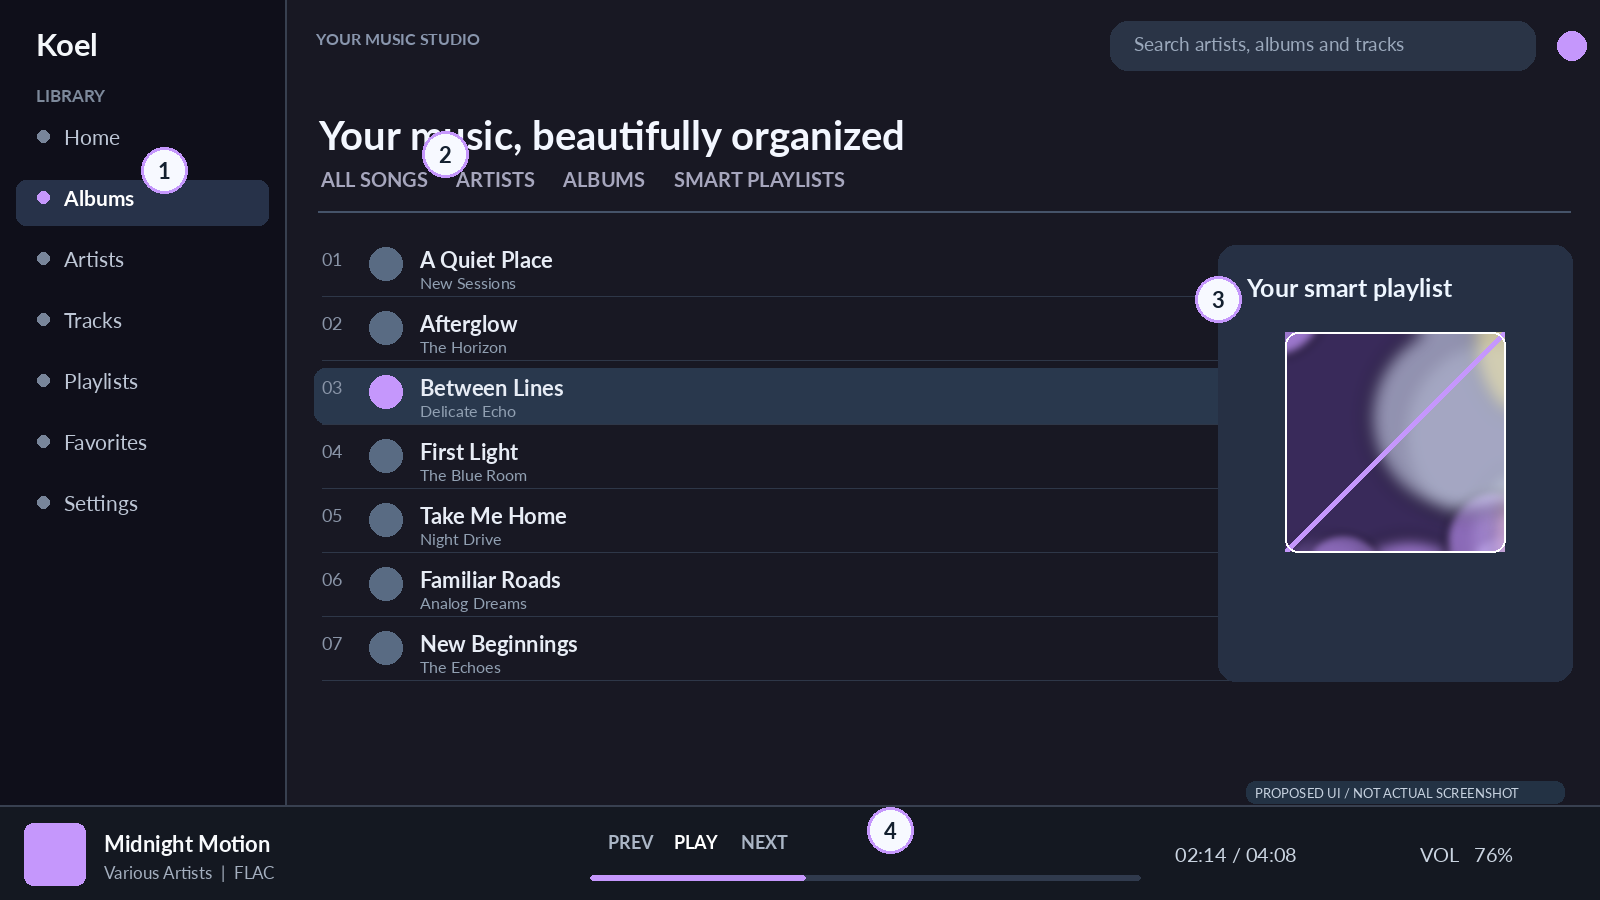
\includegraphics[width=\linewidth,height=93mm,keepaspectratio]{Music_Player_UIUX_Assets/koel_concept.png}
\end{center}
{\small\color{muted}\textit{Annotated concept:} A crisp SaaS-like library app with efficient data tables, omnipresent playback and clean empty states. Place library ownership and permissions before premium effects. \textbf{Intended platform:} Self-hosted responsive web. The visual uses invented album names and placeholder artwork.\par}
\subsection*{Proposed visual design system}
\begin{tabularx}{\linewidth}{@{}p{24mm}X@{}}
\textbf{Palette} & \colorbox[HTML]{181823}{\rule{6mm}{3mm}}\, Base 181823 \quad \colorbox[HTML]{C597FC}{\rule{6mm}{3mm}}\, Accent C597FC \\
\textbf{Typography} & Body 14--16 px; labels 12--13 px; primary screen heading 26--34 px; numeric audio data set in tabular figures.\\
\textbf{Spacing} & 4/8 px grid; 8--16 px card radius; align cover art to text blocks; 44 px touch-target minimum where relevant.\\
\textbf{Contrast} & Target WCAG AA text contrast, 4.5:1 for normal text and 3:1 for large text; verify final palette in both light/dark states.\\
\end{tabularx}
\subsection*{Annotated interface anatomy}
\begin{tabularx}{\linewidth}{@{}p{12mm}X@{}}\toprule Mark & Proposed region and responsibilities\\\midrule
\textbf{1} & Stable library navigation and smart-playlist entry points\\
\textbf{2} & Sortable catalog with multi-select and discoverable bulk actions\\
\textbf{3} & Selected song detail; contextual playlist/save operations\\
\textbf{4} & Persistent playback controls independent of route changes\\
\bottomrule\end{tabularx}
\clearpage
\section{UX functional specification [P]}
\subsection*{Information architecture and screens}
\begin{tabularx}{\linewidth}{@{}p{34mm}X@{}}\toprule Screen / route & Core content and controls\\\midrule
All Songs & Search, sort, multiselect, formats and contextual row actions\\
Artists / Albums & Artwork-centric drill-down and related media\\
Playlist manager & Create, edit, reorder, smart conditions and collaboration disclosures\\
Now playing & Queue, artwork, transport and source-quality status\\
Administration & Library scan state, account, source roots and permissions\\
\bottomrule\end{tabularx}
\subsection*{Navigation model}
Fixed desktop sidebar and responsive overlay drawer; sticky full-width playback dock with keyboard control.\par
\subsection*{Critical user journeys}
\begin{enumerate}[leftmargin=*,itemsep=3pt,topsep=2pt]
\item \textbf{Onboard library.} Configure storage; run scan; show indexing completion; offer first playlist.
\item \textbf{Build smart playlist.} Open Playlists; choose rules; preview matching results; save; revisit filters.
\item \textbf{Bulk action.} Select rows; add to playlist; confirm applied count; undo when reversible.
\end{enumerate}
\subsection*{Interaction, feedback and edge states}
Context menus also accessible by keyboard; direct drag/drop includes a menu alternative; row hover never hides only action.\par
\begin{tabularx}{\linewidth}{@{}p{39mm}X@{}}\toprule State / trigger & Expected UX behavior\\\midrule
Empty library & Offer Add music instructions and direct scanner status.\\
Authorization denied & Preserve current view; explain that action requires permission.\\
Scan failure & Report skipped paths/files and a resumable retry path.\\
\bottomrule\end{tabularx}
\subsection*{Implementation and QA contract}
\begin{itemize}[leftmargin=*,itemsep=2pt,topsep=2pt]
\item \textbf{Single source of truth.} Playback, queue and current destination/device belong to the application state model, not duplicated per view.
\item \textbf{Accessibility.} Keyboard navigation, screen-reader labels, visible focus, user-controlled lyric scrolling, reduced motion and non-color-only states.
\item \textbf{Responsive behavior.} Preserve transport when resizing; test narrow, zoomed and high-font settings; use alternative to drag-only controls.
\item \textbf{Instrumentation.} library first-play conversion; playlist create success; bulk-action reversal rate; scan recovery.
\item \textbf{Boundary.} Premium Koel Plus functions and white-label features are separately licensed: a conceptual mock does not imply they ship in MIT core.
\end{itemize}
\vspace{2mm}\begin{evidencebox}\small\textbf{Prototype acceptance:} Primary play and pause remain available through every screen; the queue and playback position survive navigation; every error has recovery text; every advertised fidelity setting accurately reflects the active engine/device. Design specifications are recommendations and require product usability testing.\end{evidencebox}
\clearpage
\chapter{Swing Music}
{\large\color{muted}Python self-hosted media service with polished browser experiences}\par
\begin{evidencebox}\small\textbf{Repository:} \sourceurl{https://github.com/swingmx/swingmusic}\\\textbf{Reference branch:} master\qquad \textbf{License:} AGPL-3.0-or-later; premium modules have separate practical availability\\\textbf{Primary stack:} Python server application; packaged local/HTTP music service; optional Android client; Docker image with mounted library/config volumes.\end{evidencebox}
\section{Observed system architecture [V]}
\begin{itemize}[leftmargin=*,itemsep=2pt,topsep=3pt]
\item Official README lists daily mixes, metadata normalization, album editions, related artists, collections, multi-user and scrobbling.
\item Documented Docker setup mounts /music and /config and exposes port 1970.
\item Dockerfile explicitly compiles premium Python modules into native extensions; their premium source is absent from the final runtime wheel.
\end{itemize}
\textbf{Visible source anchors [V].} src/swingmusic/, docs/, requirements.txt, pyproject.toml, Dockerfile, run.py.\par
\begin{evidencebox}\tagboundary{} An independently published swingmx/webclient repository exists, but its exact relationship to the current packaged browser UI was not proven. Premium internals are not represented as publicly reusable source.\end{evidencebox}
\section{Functional block blueprint [P]}
\begin{center}
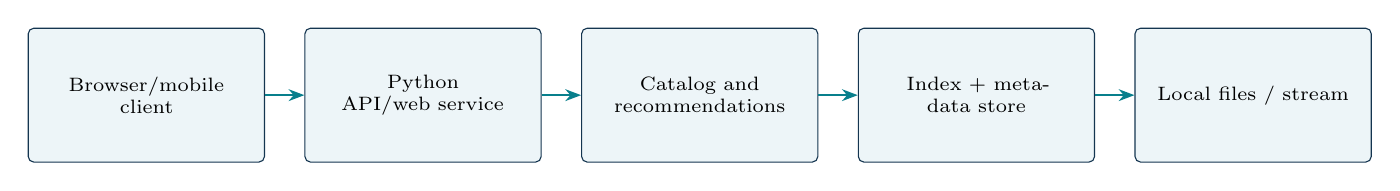
\begin{tikzpicture}[>=Stealth, node distance=1.4mm, every node/.style={font=\scriptsize,align=center}]
\node[draw=navy,rounded corners=2pt,fill=light,text width=26mm,minimum height=17mm,inner sep=2mm] (n0) {Browser/mobile client};
\node[draw=navy,rounded corners=2pt,fill=light,text width=26mm,minimum height=17mm,inner sep=2mm,right=5mm of n0] (n1) {Python API/web service};
\draw[-{Stealth[length=2mm]},thick,color=teal] (n0.east) -- (n1.west);
\node[draw=navy,rounded corners=2pt,fill=light,text width=26mm,minimum height=17mm,inner sep=2mm,right=5mm of n1] (n2) {Catalog and recommendations};
\draw[-{Stealth[length=2mm]},thick,color=teal] (n1.east) -- (n2.west);
\node[draw=navy,rounded corners=2pt,fill=light,text width=26mm,minimum height=17mm,inner sep=2mm,right=5mm of n2] (n3) {Index + metadata store};
\draw[-{Stealth[length=2mm]},thick,color=teal] (n2.east) -- (n3.west);
\node[draw=navy,rounded corners=2pt,fill=light,text width=26mm,minimum height=17mm,inner sep=2mm,right=5mm of n3] (n4) {Local files / stream};
\draw[-{Stealth[length=2mm]},thick,color=teal] (n3.east) -- (n4.west);
\end{tikzpicture}
\end{center}
\small\textit{Figure 4: Conceptual runtime path for a comparable implementation. This is not a traced source-code call graph.}\normalsize\par
\section{End-to-end user-to-speaker flow}
\begin{enumerate}[leftmargin=*,itemsep=2pt,topsep=2pt]
\item Server scans mounted local music folders.
\item Metadata service normalizes records, related albums and editions.
\item The client requests library views, cover art and curated mix listings.
\item Audio route serves local or processed audio to the selected client.
\item Listening events update history and may feed the next daily mix.
\end{enumerate}
\section{Data contract [P]}
\begin{evidencebox}\small\textbf{Candidate conceptual entities (not copied database classes):}\par
\begin{itemize}[leftmargin=*,itemsep=1pt,topsep=2pt]
\item \texttt{AudioFile(path, checksum, tags)}
\item \texttt{CanonicalAlbum(id, edition\_label)}
\item \texttt{ArtistRelationship(src\_id, dst\_id, kind)}
\item \texttt{ListeningHistory(user, track, played\_at)}
\item \texttt{MixSnapshot(user, generated\_at, track\_ids)}
\end{itemize}\end{evidencebox}
\section{Implementation blueprint [P]}
\begin{itemize}[leftmargin=*,itemsep=2pt,topsep=3pt]
\item Separate scanner, normalization, album-version resolver and recommendation worker for predictable updates.
\item Use an explicit LocalMediaRepository with checked path roots and atomic incremental index updates.
\item Implement mix generation as an offline scheduled computation with recorded version, inputs and reproducible seed.
\item Give browser player and Android client a stable documented API and paginated library endpoints.
\item Track audio transitions as a policy (silence detection, crossfade) and allow a fidelity mode that disables DSP.
\item Separate publicly available AGPL server code from any compiled or independently licensed premium feature.
\end{itemize}
\subsection*{Engineering equation}
\begin{equation*}\mathrm{Score}(u,t)=\alpha\,\mathrm{Affinity}(u,t)+\beta\,\mathrm{Novelty}(t)-\gamma\,\mathrm{RepeatPenalty}(u,t)\end{equation*}
A suggested recommendation score for a comparable product; it is not claimed as Swing Music's actual recommendation algorithm.\par
\section{Validation and operational guardrails}
\textbf{Acceptance-test plan [P].}\par
\begin{itemize}[leftmargin=*,itemsep=2pt,topsep=3pt]
\item Reproducible daily-mix test snapshots and sparse-history fallback.
\item Server concurrency and seek behavior with multiple accounts.
\item Metadata normalization golden files for deluxe/remaster editions.
\end{itemize}
\textbf{Constraints and risks [B].}\par
\begin{itemize}[leftmargin=*,itemsep=2pt,topsep=3pt]
\item AGPL network-service obligations require careful review for modified deployments.
\item Premium compiled components should not be assumed reusable from public Python sources.
\item Mobile and browser clients may differ in crossfade and decoding capability.
\end{itemize}
\section*{Primary evidence and source entry points}
\begin{itemize}[leftmargin=*,itemsep=1pt,topsep=1pt]
\item \sourceurl{https://github.com/swingmx/swingmusic}
\item \sourceurl{https://github.com/swingmx/swingmusic/blob/master/Dockerfile}
\item \sourceurl{https://github.com/swingmx/webclient}
\end{itemize}
\clearpage
\section{UI/UX architecture and annotated screen concept}
\begin{evidencebox}\small\tagverified{} The official website shows Home, Folder Browser, Album, Artist, Now Playing, Lyrics, Favorites and Collections. Its README lists daily mixes, related albums, listening statistics, silence detection and multiuser support.\\[2pt]\textbf{UX evidence link:} \sourceurl{https://swingmx.com/}\\[2pt]\tagproposal{} The image, colors, exact screen compositions, flows, and acceptance criteria below are authored design recommendations, not release screenshots or audited internal UI components.\end{evidencebox}
\begin{center}
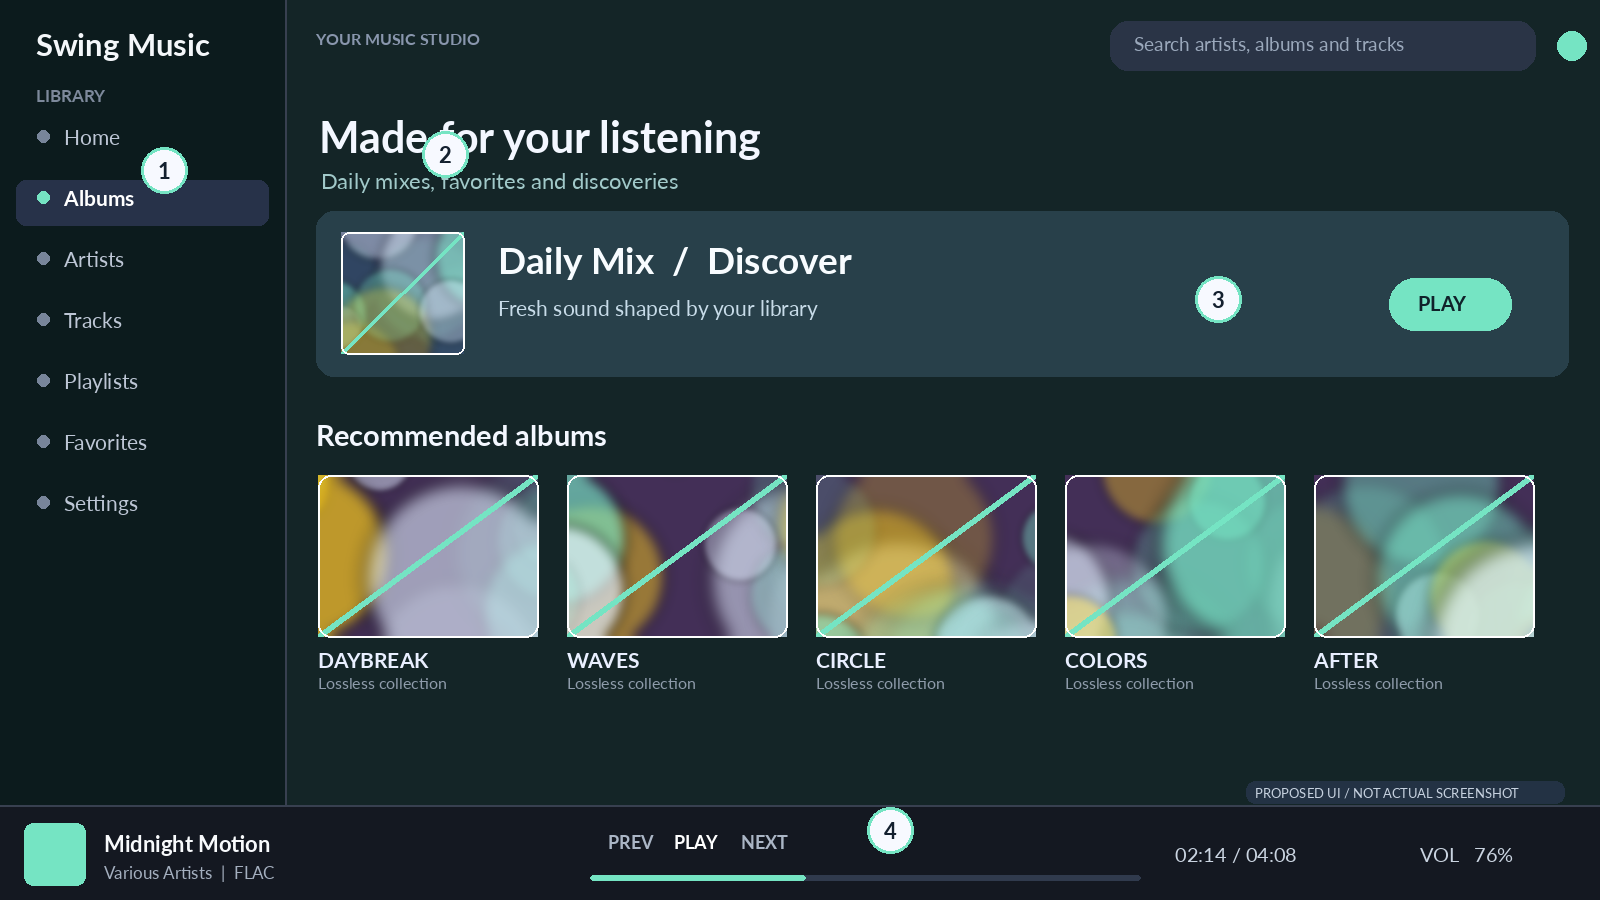
\includegraphics[width=\linewidth,height=93mm,keepaspectratio]{Music_Player_UIUX_Assets/swing_music_concept.png}
\end{center}
{\small\color{muted}\textit{Annotated concept:} Streaming-service-inspired editorial discovery: hero cards, curated mixes, album collections and visual consumption history. \textbf{Intended platform:} Self-hosted browser + client. The visual uses invented album names and placeholder artwork.\par}
\subsection*{Proposed visual design system}
\begin{tabularx}{\linewidth}{@{}p{24mm}X@{}}
\textbf{Palette} & \colorbox[HTML]{142527}{\rule{6mm}{3mm}}\, Base 142527 \quad \colorbox[HTML]{75E4C3}{\rule{6mm}{3mm}}\, Accent 75E4C3 \\
\textbf{Typography} & Body 14--16 px; labels 12--13 px; primary screen heading 26--34 px; numeric audio data set in tabular figures.\\
\textbf{Spacing} & 4/8 px grid; 8--16 px card radius; align cover art to text blocks; 44 px touch-target minimum where relevant.\\
\textbf{Contrast} & Target WCAG AA text contrast, 4.5:1 for normal text and 3:1 for large text; verify final palette in both light/dark states.\\
\end{tabularx}
\subsection*{Annotated interface anatomy}
\begin{tabularx}{\linewidth}{@{}p{12mm}X@{}}\toprule Mark & Proposed region and responsibilities\\\midrule
\textbf{1} & Global For You, Folder and Collection destinations\\
\textbf{2} & Personalized daily-mix hero with disclosed data basis\\
\textbf{3} & Recommended album cards and efficient single-click play\\
\textbf{4} & Persistent playback bar plus direct queue access\\
\bottomrule\end{tabularx}
\clearpage
\section{UX functional specification [P]}
\subsection*{Information architecture and screens}
\begin{tabularx}{\linewidth}{@{}p{34mm}X@{}}\toprule Screen / route & Core content and controls\\\midrule
For You / Daily Mixes & Personalized cards, recent listening and quick play\\
Folder Browser & Literal folder path navigation for users who think in files\\
Artists / Albums & Editorial covers, versions and related works\\
Now Playing + Lyrics & Immersive listening and queue, with discreet utility controls\\
Statistics / Collections & History, favorites and manually grouped albums\\
\bottomrule\end{tabularx}
\subsection*{Navigation model}
Discover / Library / Folders / Collections global entries; contextual artist, album and track sheets.\par
\subsection*{Critical user journeys}
\begin{enumerate}[leftmargin=*,itemsep=3pt,topsep=2pt]
\item \textbf{Start daily mix.} Home; inspect mix provenance; play; save related artist; return Home.
\item \textbf{Find folder file.} Open Folders; expand source root; queue local track; return to browsing.
\item \textbf{Crossfade disclosure.} Set fade preference; preview; show silence-detection effect near controls.
\end{enumerate}
\subsection*{Interaction, feedback and edge states}
Card hover surfaces quick play with visible focus; queue insert feedback; statistics date range and clear privacy information.\par
\begin{tabularx}{\linewidth}{@{}p{39mm}X@{}}\toprule State / trigger & Expected UX behavior\\\midrule
Recommendation not ready & Display Recent Plays rather than generic duplicate content.\\
Silence trimming active & Show an explicit processing label with a toggle; avoid surprising cuts.\\
Version ambiguity & Show album edition/year label so duplicates remain intelligible.\\
\bottomrule\end{tabularx}
\subsection*{Implementation and QA contract}
\begin{itemize}[leftmargin=*,itemsep=2pt,topsep=2pt]
\item \textbf{Single source of truth.} Playback, queue and current destination/device belong to the application state model, not duplicated per view.
\item \textbf{Accessibility.} Keyboard navigation, screen-reader labels, visible focus, user-controlled lyric scrolling, reduced motion and non-color-only states.
\item \textbf{Responsive behavior.} Preserve transport when resizing; test narrow, zoomed and high-font settings; use alternative to drag-only controls.
\item \textbf{Instrumentation.} daily-mix engagement; path-to-play; discover-to-save; unexpected skip feedback.
\item \textbf{Boundary.} Confirm source availability of premium features before adapting; some release packaging includes non-plain-source modules.
\end{itemize}
\vspace{2mm}\begin{evidencebox}\small\textbf{Prototype acceptance:} Primary play and pause remain available through every screen; the queue and playback position survive navigation; every error has recovery text; every advertised fidelity setting accurately reflects the active engine/device. Design specifications are recommendations and require product usability testing.\end{evidencebox}
\clearpage
\chapter{Museeks}
{\large\color{muted}Lean cross-platform Tauri music player}\par
\begin{evidencebox}\small\textbf{Repository:} \sourceurl{https://github.com/martpie/museeks}\\\textbf{Reference branch:} master\qquad \textbf{License:} MIT\\\textbf{Primary stack:} Tauri v2 / Rust native shell; React UI; Vite/TypeScript; local file player.\end{evidencebox}
\section{Observed system architecture [V]}
\begin{itemize}[leftmargin=*,itemsep=2pt,topsep=3pt]
\item README documents a Tauri v2 Rust backend and React frontend.
\item Feature set includes local FLAC/WAV/MP3, playlists, queue, cover art, auto-refresh, M3U import/export and playback speed.
\item Build instructions use the Tauri dev workflow and frontend hot reloading.
\end{itemize}
\textbf{Visible source anchors [V].} src/, src-tauri/, scripts/, package.json, vite.config.ts, pnpm-workspace.yaml.\par
\begin{evidencebox}\tagboundary{} The proposed Rust command names and data model are reference design contracts, not confirmed Museeks public function identifiers.\end{evidencebox}
\section{Functional block blueprint [P]}
\begin{center}
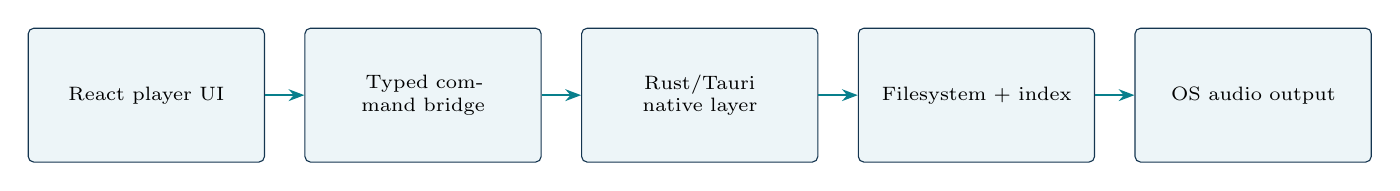
\begin{tikzpicture}[>=Stealth, node distance=1.4mm, every node/.style={font=\scriptsize,align=center}]
\node[draw=navy,rounded corners=2pt,fill=light,text width=26mm,minimum height=17mm,inner sep=2mm] (n0) {React player UI};
\node[draw=navy,rounded corners=2pt,fill=light,text width=26mm,minimum height=17mm,inner sep=2mm,right=5mm of n0] (n1) {Typed command bridge};
\draw[-{Stealth[length=2mm]},thick,color=teal] (n0.east) -- (n1.west);
\node[draw=navy,rounded corners=2pt,fill=light,text width=26mm,minimum height=17mm,inner sep=2mm,right=5mm of n1] (n2) {Rust/Tauri native layer};
\draw[-{Stealth[length=2mm]},thick,color=teal] (n1.east) -- (n2.west);
\node[draw=navy,rounded corners=2pt,fill=light,text width=26mm,minimum height=17mm,inner sep=2mm,right=5mm of n2] (n3) {Filesystem + index};
\draw[-{Stealth[length=2mm]},thick,color=teal] (n2.east) -- (n3.west);
\node[draw=navy,rounded corners=2pt,fill=light,text width=26mm,minimum height=17mm,inner sep=2mm,right=5mm of n3] (n4) {OS audio output};
\draw[-{Stealth[length=2mm]},thick,color=teal] (n3.east) -- (n4.west);
\end{tikzpicture}
\end{center}
\small\textit{Figure 5: Conceptual runtime path for a comparable implementation. This is not a traced source-code call graph.}\normalsize\par
\section{End-to-end user-to-speaker flow}
\begin{enumerate}[leftmargin=*,itemsep=2pt,topsep=2pt]
\item User chooses one or more local folders.
\item Native layer scans supported audio and exposes metadata to the React catalog.
\item Queue changes in the UI produce a typed command to the native playback layer.
\item Audio decoder/device handles playback while a state channel updates the player screen.
\item Playlist and preferences persist locally and can be exported as M3U where supported.
\end{enumerate}
\section{Data contract [P]}
\begin{evidencebox}\small\textbf{Candidate conceptual entities (not copied database classes):}\par
\begin{itemize}[leftmargin=*,itemsep=1pt,topsep=2pt]
\item \texttt{LibraryRoot(path, watch\_enabled)}
\item \texttt{Track(id, uri, duration, tags)}
\item \texttt{Playlist(id, name); Entry(track\_id, pos)}
\item \texttt{NowPlaying(track\_id, position\_ms)}
\item \texttt{Preferences(theme, output, playback\_speed)}
\end{itemize}\end{evidencebox}
\section{Implementation blueprint [P]}
\begin{itemize}[leftmargin=*,itemsep=2pt,topsep=3pt]
\item Preserve the small deployable: Rust owns file access and OS integrations; React owns visualization and interaction.
\item Use typed bridge commands and typed native events; validate URIs so the frontend cannot open arbitrary hidden files.
\item Extract a LibraryService, PlaylistService and PlaybackService before adding new cloud or streaming features.
\item Use a stable track identity strategy for renames and library refresh; keep broken files as recoverable scan errors.
\item Build theme tokens, cover-art components and keyboard accessibility first for a premium redesign.
\item Add explicit fidelity and audio-device settings only if supported by the chosen playback dependency.
\end{itemize}
\subsection*{Engineering equation}
\begin{equation*}\mathrm{RefreshCost}=O(N_{\mathrm{changed}})+O(N_{\mathrm{watch\ events}})\end{equation*}
The target is an incremental watcher/indexer rather than an unconditional full-library rescan.\par
\section{Validation and operational guardrails}
\textbf{Acceptance-test plan [P].}\par
\begin{itemize}[leftmargin=*,itemsep=2pt,topsep=3pt]
\item Cross-platform file picker and permission tests on Linux, macOS and Windows.
\item Large library and M3U import/export tests including missing tracks.
\item Audio continuity while UI navigates or theme settings change.
\end{itemize}
\textbf{Constraints and risks [B].}\par
\begin{itemize}[leftmargin=*,itemsep=2pt,topsep=3pt]
\item Tauri bridge and OS decoder capabilities vary by platform.
\item Lossless FLAC support is not a guarantee of bit-perfect DAC output.
\item Code is MIT but third-party decoder/license obligations still apply.
\end{itemize}
\section*{Primary evidence and source entry points}
\begin{itemize}[leftmargin=*,itemsep=1pt,topsep=1pt]
\item \sourceurl{https://github.com/martpie/museeks}
\item \sourceurl{https://github.com/martpie/museeks/blob/master/README.md}
\end{itemize}
\clearpage
\section{UI/UX architecture and annotated screen concept}
\begin{evidencebox}\small\tagverified{} The README confirms a local cross-platform player with React UI, Tauri/Rust backend, cover art, playlists, queue, dark theme, playback speed and M3U import/export.\\[2pt]\textbf{UX evidence link:} \sourceurl{https://github.com/martpie/museeks}\\[2pt]\tagproposal{} The image, colors, exact screen compositions, flows, and acceptance criteria below are authored design recommendations, not release screenshots or audited internal UI components.\end{evidencebox}
\begin{center}
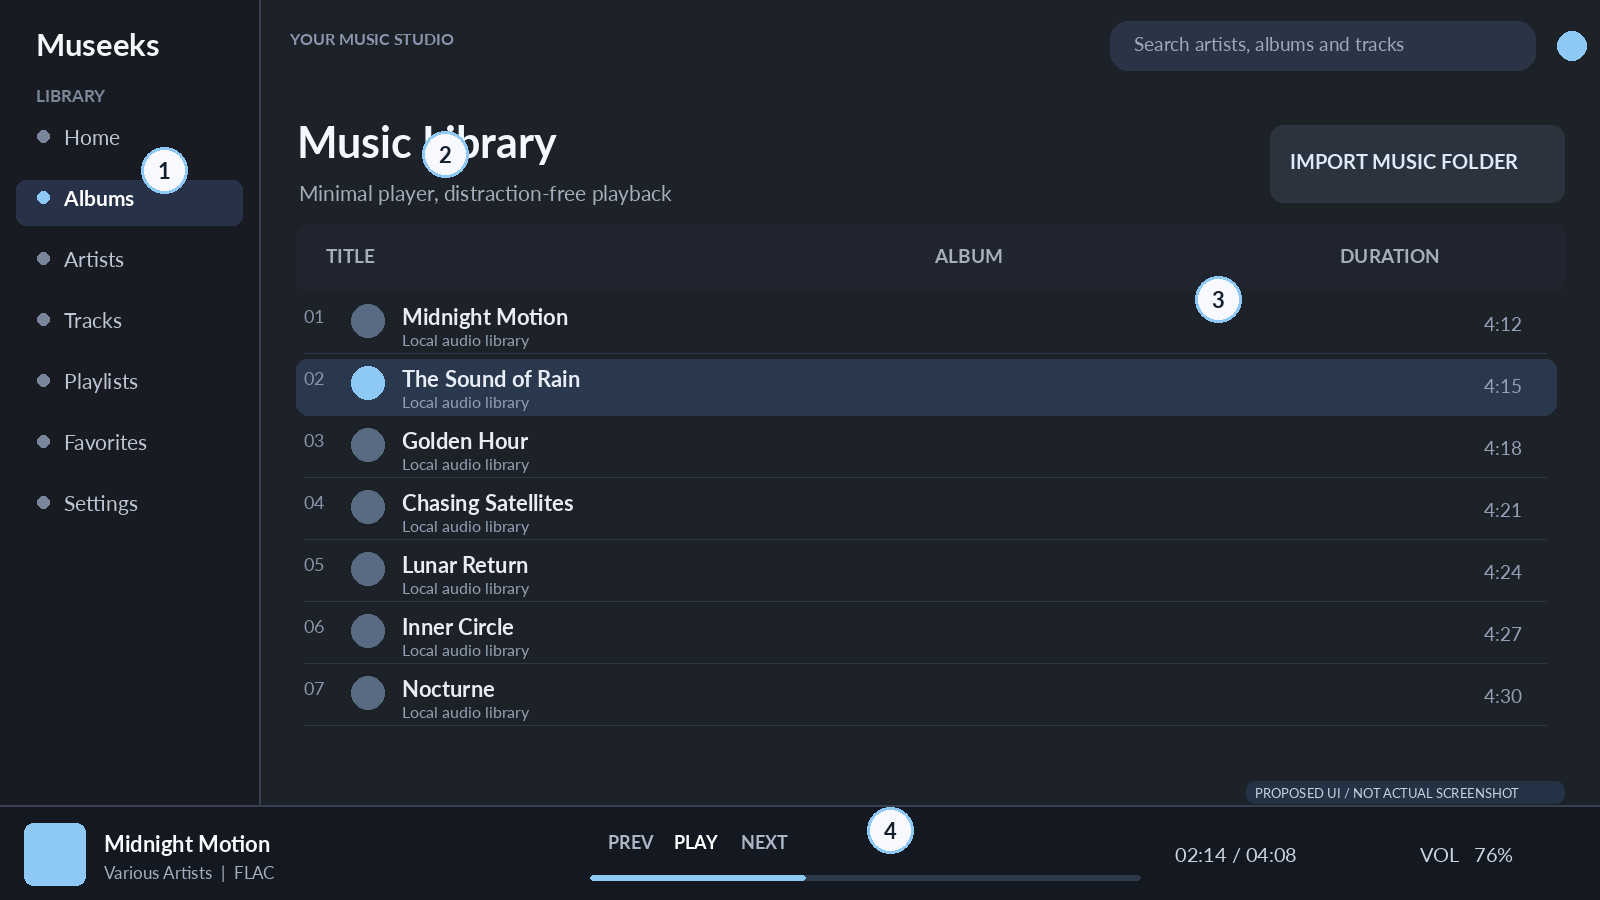
\includegraphics[width=\linewidth,height=93mm,keepaspectratio]{Music_Player_UIUX_Assets/museeks_concept.png}
\end{center}
{\small\color{muted}\textit{Annotated concept:} Minimalist, native-feeling library with one strong primary task: choosing and playing local music. Avoid dashboard bloat. \textbf{Intended platform:} Tauri desktop. The visual uses invented album names and placeholder artwork.\par}
\subsection*{Proposed visual design system}
\begin{tabularx}{\linewidth}{@{}p{24mm}X@{}}
\textbf{Palette} & \colorbox[HTML]{1D2128}{\rule{6mm}{3mm}}\, Base 1D2128 \quad \colorbox[HTML]{8EC9F6}{\rule{6mm}{3mm}}\, Accent 8EC9F6 \\
\textbf{Typography} & Body 14--16 px; labels 12--13 px; primary screen heading 26--34 px; numeric audio data set in tabular figures.\\
\textbf{Spacing} & 4/8 px grid; 8--16 px card radius; align cover art to text blocks; 44 px touch-target minimum where relevant.\\
\textbf{Contrast} & Target WCAG AA text contrast, 4.5:1 for normal text and 3:1 for large text; verify final palette in both light/dark states.\\
\end{tabularx}
\subsection*{Annotated interface anatomy}
\begin{tabularx}{\linewidth}{@{}p{12mm}X@{}}\toprule Mark & Proposed region and responsibilities\\\midrule
\textbf{1} & Minimal navigation for import, library and playlists\\
\textbf{2} & High-density track table with keyboard-friendly sorting\\
\textbf{3} & Import/sync affordances without unnecessary editorial panels\\
\textbf{4} & Pinned transport with clear local-file status\\
\bottomrule\end{tabularx}
\clearpage
\section{UX functional specification [P]}
\subsection*{Information architecture and screens}
\begin{tabularx}{\linewidth}{@{}p{34mm}X@{}}\toprule Screen / route & Core content and controls\\\midrule
First-run Import & Folder picker, format support and indexing feedback\\
Library / Songs & Dense searchable table, stable selected row and sort\\
Playlists & Import/export M3U, reordering and missing-file handling\\
Mini player & Transport, queue, volume, source label and playback speed\\
Preferences & Theme, scan roots, audio availability and shortcuts\\
\bottomrule\end{tabularx}
\subsection*{Navigation model}
Two-pane desktop window with short sidebar, searchable list and pinned transport. Do not require more than two clicks for primary playback.\par
\subsection*{Critical user journeys}
\begin{enumerate}[leftmargin=*,itemsep=3pt,topsep=2pt]
\item \textbf{Add folder.} Open library settings; approve OS folder permission; index incremental changes.
\item \textbf{Play queue.} Select multiple tracks; add to queue; rearrange; save as playlist.
\item \textbf{Import playlist.} Read M3U; match local paths; show unmatched tracks; allow correction.
\end{enumerate}
\subsection*{Interaction, feedback and edge states}
Native file drag/drop, OS keyboard shortcuts, accessible table sorting and persistent queue across route changes.\par
\begin{tabularx}{\linewidth}{@{}p{39mm}X@{}}\toprule State / trigger & Expected UX behavior\\\midrule
No music & Use a single prominent Open Folder CTA with codec explanation.\\
Missing file & Keep list position; explain missing path; offer Locate or Skip.\\
Watch permission revoked & Show stale library banner and fix-in-settings flow.\\
\bottomrule\end{tabularx}
\subsection*{Implementation and QA contract}
\begin{itemize}[leftmargin=*,itemsep=2pt,topsep=2pt]
\item \textbf{Single source of truth.} Playback, queue and current destination/device belong to the application state model, not duplicated per view.
\item \textbf{Accessibility.} Keyboard navigation, screen-reader labels, visible focus, user-controlled lyric scrolling, reduced motion and non-color-only states.
\item \textbf{Responsive behavior.} Preserve transport when resizing; test narrow, zoomed and high-font settings; use alternative to drag-only controls.
\item \textbf{Instrumentation.} folder import time; library refresh lag; M3U resolution; time-to-play; playback command latency.
\item \textbf{Boundary.} Tauri bridge permissions and audio capabilities vary by host OS and third-party native modules.
\end{itemize}
\vspace{2mm}\begin{evidencebox}\small\textbf{Prototype acceptance:} Primary play and pause remain available through every screen; the queue and playback position survive navigation; every error has recovery text; every advertised fidelity setting accurately reflects the active engine/device. Design specifications are recommendations and require product usability testing.\end{evidencebox}
\clearpage
\chapter{Strawberry}
{\large\color{muted}Audiophile-focused Qt desktop library and playback system}\par
\begin{evidencebox}\small\textbf{Repository:} \sourceurl{https://github.com/strawberrymusicplayer/strawberry}\\\textbf{Reference branch:} master\qquad \textbf{License:} GPL-3.0\\\textbf{Primary stack:} C++ / Qt application; native library management; decoder/playback subsystem; metadata and loudness tooling.\end{evidencebox}
\section{Observed system architecture [V]}
\begin{itemize}[leftmargin=*,itemsep=2pt,topsep=3pt]
\item README explicitly identifies Qt/C++ and extensive lossless formats including FLAC, ALAC, WavPack and DSD.
\item Advanced features include Linux bit-perfect output, ReplayGain/EBU R128, waveform, tag editing and audio analyzer.
\item Codebase is organized as a CMake desktop project with a src tree and tests.
\end{itemize}
\textbf{Visible source anchors [V].} src/, tests/, data/, CMakeLists.txt, cmake/, dist/.\par
\begin{evidencebox}\tagboundary{} Exact audio backend plugin call graph was not traced. The proposed processing stages illustrate an audiophile-safe architecture rather than asserting a fixed order in Strawberry.\end{evidencebox}
\section{Functional block blueprint [P]}
\begin{center}
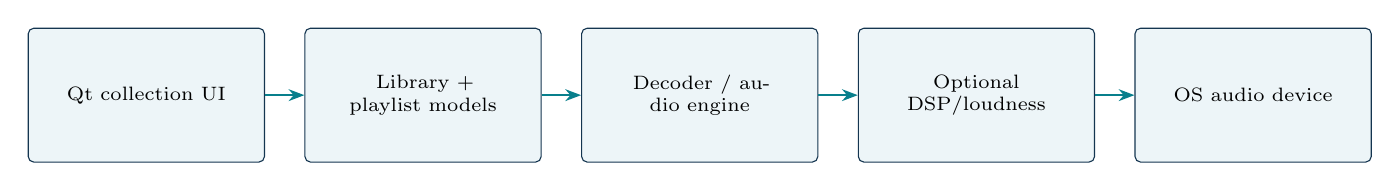
\begin{tikzpicture}[>=Stealth, node distance=1.4mm, every node/.style={font=\scriptsize,align=center}]
\node[draw=navy,rounded corners=2pt,fill=light,text width=26mm,minimum height=17mm,inner sep=2mm] (n0) {Qt collection UI};
\node[draw=navy,rounded corners=2pt,fill=light,text width=26mm,minimum height=17mm,inner sep=2mm,right=5mm of n0] (n1) {Library + playlist models};
\draw[-{Stealth[length=2mm]},thick,color=teal] (n0.east) -- (n1.west);
\node[draw=navy,rounded corners=2pt,fill=light,text width=26mm,minimum height=17mm,inner sep=2mm,right=5mm of n1] (n2) {Decoder / audio engine};
\draw[-{Stealth[length=2mm]},thick,color=teal] (n1.east) -- (n2.west);
\node[draw=navy,rounded corners=2pt,fill=light,text width=26mm,minimum height=17mm,inner sep=2mm,right=5mm of n2] (n3) {Optional DSP/loudness};
\draw[-{Stealth[length=2mm]},thick,color=teal] (n2.east) -- (n3.west);
\node[draw=navy,rounded corners=2pt,fill=light,text width=26mm,minimum height=17mm,inner sep=2mm,right=5mm of n3] (n4) {OS audio device};
\draw[-{Stealth[length=2mm]},thick,color=teal] (n3.east) -- (n4.west);
\end{tikzpicture}
\end{center}
\small\textit{Figure 6: Conceptual runtime path for a comparable implementation. This is not a traced source-code call graph.}\normalsize\par
\section{End-to-end user-to-speaker flow}
\begin{enumerate}[leftmargin=*,itemsep=2pt,topsep=2pt]
\item Scanner indexes audio collections and retrieves embedded/external metadata.
\item User filters library or loads a dynamic playlist.
\item Playback engine selects a decoder and compatible output format.
\item If enabled, normalization or EQ processes samples; otherwise the untouched path is preferred.
\item Audio device plays decoded samples and surfaces analyzer/position data.
\end{enumerate}
\section{Data contract [P]}
\begin{evidencebox}\small\textbf{Candidate conceptual entities (not copied database classes):}\par
\begin{itemize}[leftmargin=*,itemsep=1pt,topsep=2pt]
\item \texttt{Track(audio\_uri, codec, sample\_rate, bit\_depth)}
\item \texttt{TagRevision(track\_id, old\_tags, new\_tags)}
\item \texttt{PlaylistMembership(list\_id, track\_id, order)}
\item \texttt{AudioPath(input\_format, output\_format, dsp\_flags)}
\item \texttt{DeviceCaps(name, rates, formats, exclusive\_mode)}
\end{itemize}\end{evidencebox}
\section{Implementation blueprint [P]}
\begin{itemize}[leftmargin=*,itemsep=2pt,topsep=3pt]
\item Keep album/tag/catalog operations independent from a strongly typed AudioEngine facade.
\item Include a device-capability probe that reports supported sample rates, formats and exclusive output support.
\item Distinguish lossless decode, DSP-off and mathematically bit-perfect output in settings and diagnostics.
\item Implement ReplayGain and EBU R128 as explicit optional processing nodes, not invisible quality claims.
\item Capture decoder, resampler and output device settings in a per-session processing manifest.
\item Automate golden-file decoding, silent-output tests and short-buffer/underrun stress tests.
\end{itemize}
\subsection*{Engineering equation}
\begin{equation*}\mathrm{BitPerfect}=\bigl(\forall n:\ y[n]=x[n]\bigr)\land(f_{s,\mathrm{out}}=f_{s,\mathrm{src}})\end{equation*}
At the PCM handoff boundary, sample identity and rate equality are necessary tests; actual hardware exclusivity is platform-dependent.\par
\section{Validation and operational guardrails}
\textbf{Acceptance-test plan [P].}\par
\begin{itemize}[leftmargin=*,itemsep=2pt,topsep=3pt]
\item Reference PCM hashing where the backend supports bypass/transparent output.
\item ReplayGain-off versus ReplayGain-on fixtures and EBU R128 comparisons.
\item Device hotplug, DSD path and library corruption regression tests.
\end{itemize}
\textbf{Constraints and risks [B].}\par
\begin{itemize}[leftmargin=*,itemsep=2pt,topsep=3pt]
\item Audiophile options should not be silently enabled because they can alter output samples.
\item Platform-specific bit-perfect claims must be validated on each OS/audio API.
\item GPL-3.0 and codec dependencies affect redistribution.
\end{itemize}
\section*{Primary evidence and source entry points}
\begin{itemize}[leftmargin=*,itemsep=1pt,topsep=1pt]
\item \sourceurl{https://github.com/strawberrymusicplayer/strawberry}
\item \sourceurl{https://github.com/strawberrymusicplayer/strawberry/blob/master/README.md}
\end{itemize}
\clearpage
\section{UI/UX architecture and annotated screen concept}
\begin{evidencebox}\small\tagverified{} Project documentation lists collection organization, playlists, waveform seek bar, analyzer, equalizer, ReplayGain/EBU R128, many lossless codecs and Linux bit-perfect playback.\\[2pt]\textbf{UX evidence link:} \sourceurl{https://github.com/strawberrymusicplayer/strawberry}\\[2pt]\tagproposal{} The image, colors, exact screen compositions, flows, and acceptance criteria below are authored design recommendations, not release screenshots or audited internal UI components.\end{evidencebox}
\begin{center}
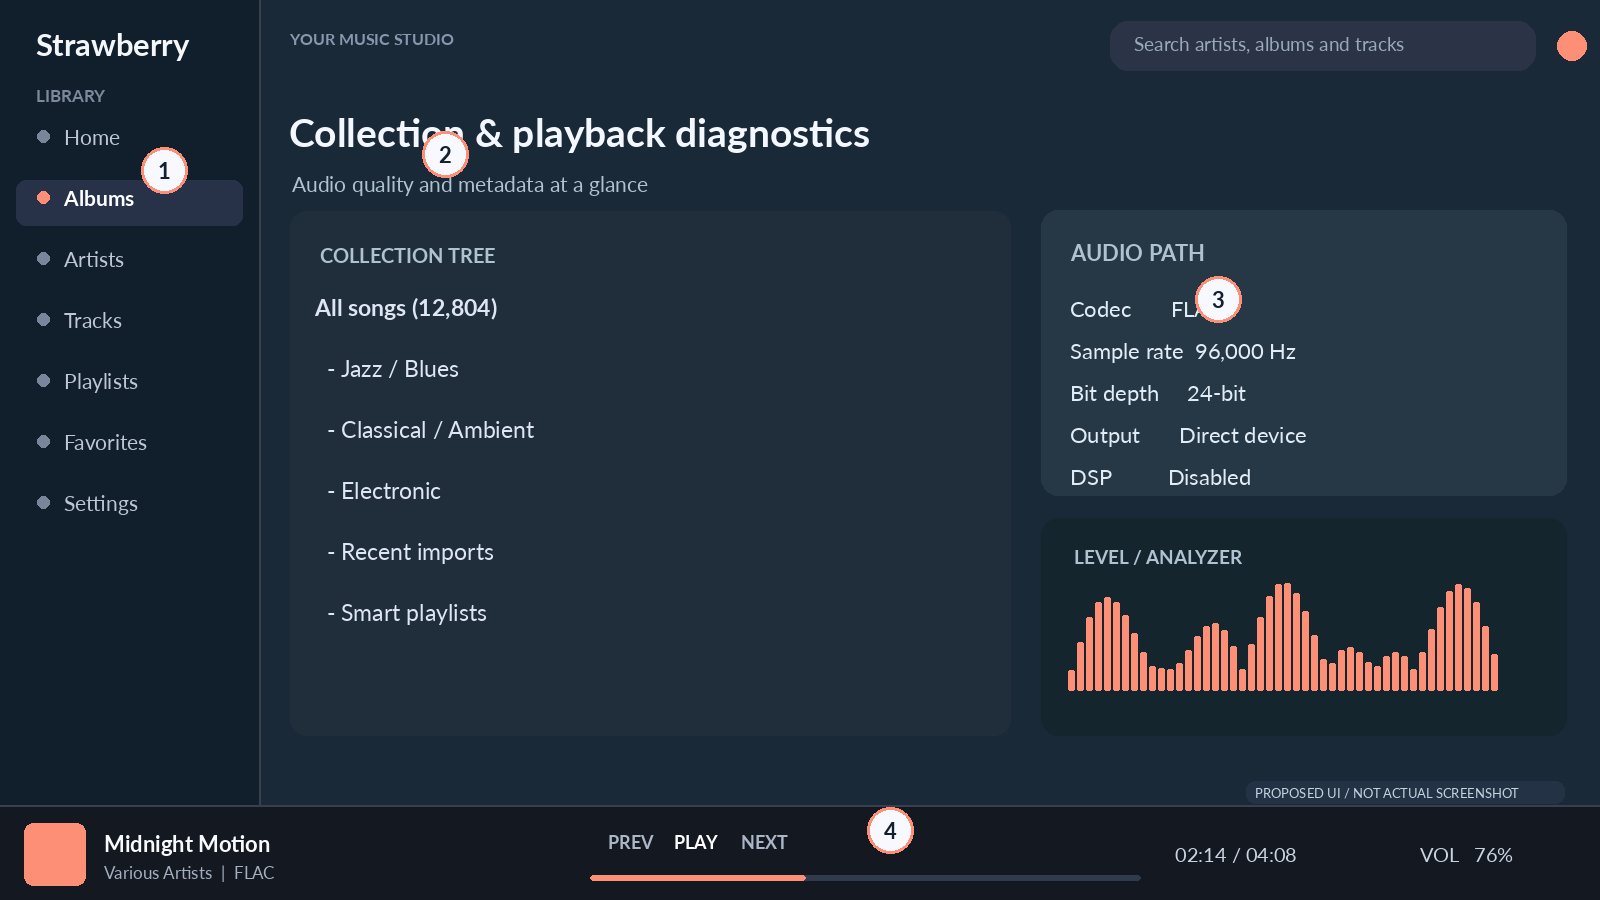
\includegraphics[width=\linewidth,height=93mm,keepaspectratio]{Music_Player_UIUX_Assets/strawberry_concept.png}
\end{center}
{\small\color{muted}\textit{Annotated concept:} Power-user desktop workspace. Keep dense metadata useful and advanced audio configuration accessible without masking signal modifications. \textbf{Intended platform:} Qt desktop. The visual uses invented album names and placeholder artwork.\par}
\subsection*{Proposed visual design system}
\begin{tabularx}{\linewidth}{@{}p{24mm}X@{}}
\textbf{Palette} & \colorbox[HTML]{1A2938}{\rule{6mm}{3mm}}\, Base 1A2938 \quad \colorbox[HTML]{FD8F76}{\rule{6mm}{3mm}}\, Accent FD8F76 \\
\textbf{Typography} & Body 14--16 px; labels 12--13 px; primary screen heading 26--34 px; numeric audio data set in tabular figures.\\
\textbf{Spacing} & 4/8 px grid; 8--16 px card radius; align cover art to text blocks; 44 px touch-target minimum where relevant.\\
\textbf{Contrast} & Target WCAG AA text contrast, 4.5:1 for normal text and 3:1 for large text; verify final palette in both light/dark states.\\
\end{tabularx}
\subsection*{Annotated interface anatomy}
\begin{tabularx}{\linewidth}{@{}p{12mm}X@{}}\toprule Mark & Proposed region and responsibilities\\\midrule
\textbf{1} & Expandable source and collection hierarchy\\
\textbf{2} & Audio library/playlist workspace with power-user control\\
\textbf{3} & Audio path details: format, output and DSP states\\
\textbf{4} & Player control and current quality report must agree\\
\bottomrule\end{tabularx}
\clearpage
\section{UX functional specification [P]}
\subsection*{Information architecture and screens}
\begin{tabularx}{\linewidth}{@{}p{34mm}X@{}}\toprule Screen / route & Core content and controls\\\midrule
Collection tree & Library roots, filters, metadata and tag editing\\
Playlist workspace & Drag/drop, advanced sorting, smart rules and queue\\
Now playing + analyzer & Waveform seek, spectrogram/levels and transport\\
Audio signal inspector & Input codec, bit depth, sample rate, DSP and device routing\\
Devices / DSP & Output device chooser, exclusive mode if supported, EQ and loudness flags\\
\bottomrule\end{tabularx}
\subsection*{Navigation model}
Resizable three-pane collection, playlist and details layout; persist pane sizes and support compact control mode.\par
\subsection*{Critical user journeys}
\begin{enumerate}[leftmargin=*,itemsep=3pt,topsep=2pt]
\item \textbf{Inspect fidelity.} Start FLAC; open output inspector; review codec/format; enable/disable DSP knowingly.
\item \textbf{Retag collection.} Select tracks; edit fields; preview; commit; log errors and undo supported edits.
\item \textbf{Choose device.} Select output device; show capabilities; warn if resampling is applied.
\end{enumerate}
\subsection*{Interaction, feedback and edge states}
Keyboard-usable tree view, semantic analyzer controls, waveform seek with accessible time alternative and signal-path disclosure.\par
\begin{tabularx}{\linewidth}{@{}p{39mm}X@{}}\toprule State / trigger & Expected UX behavior\\\midrule
Device disconnect & Pause/fallback with explicit route notice; never silently claim bit-perfect.\\
Metadata lookup fails & Retain original tags and offer manual entry.\\
Unsupported format & Display codec explanation and actionable installation path when relevant.\\
\bottomrule\end{tabularx}
\subsection*{Implementation and QA contract}
\begin{itemize}[leftmargin=*,itemsep=2pt,topsep=2pt]
\item \textbf{Single source of truth.} Playback, queue and current destination/device belong to the application state model, not duplicated per view.
\item \textbf{Accessibility.} Keyboard navigation, screen-reader labels, visible focus, user-controlled lyric scrolling, reduced motion and non-color-only states.
\item \textbf{Responsive behavior.} Preserve transport when resizing; test narrow, zoomed and high-font settings; use alternative to drag-only controls.
\item \textbf{Instrumentation.} unexpected format conversions; output-device switches; tag-write failures; under-run events; screen-reader playback discoverability.
\item \textbf{Boundary.} Theoretical bit-perfect mode must be reported as tested per platform, sink and configuration; not guaranteed by a displayed FLAC badge.
\end{itemize}
\vspace{2mm}\begin{evidencebox}\small\textbf{Prototype acceptance:} Primary play and pause remain available through every screen; the queue and playback position survive navigation; every error has recovery text; every advertised fidelity setting accurately reflects the active engine/device. Design specifications are recommendations and require product usability testing.\end{evidencebox}
\clearpage
\chapter{Finamp}
{\large\color{muted}Flutter Jellyfin client with durable offline playback}\par
\begin{evidencebox}\small\textbf{Repository:} \sourceurl{https://github.com/finamp-app/finamp}\\\textbf{Reference branch:} redesign\qquad \textbf{License:} MPL-2.0\\\textbf{Primary stack:} Flutter/Dart mobile/desktop UI; Jellyfin API service; local downloads; playback engine and platform integrations.\end{evidencebox}
\section{Observed system architecture [V]}
\begin{itemize}[leftmargin=*,itemsep=2pt,topsep=3pt]
\item Finamp is a Jellyfin music client for mobile and desktop, with gapless playback, offline downloads and transcoded streams.
\item README documents dynamic themes, lyrics, ReplayGain, Android Auto and CarPlay.
\item Source structure is a cross-platform Flutter application with automated tests and platform directories.
\end{itemize}
\textbf{Visible source anchors [V].} lib/, android/, ios/, linux/, macos/, windows/, integration\_test/, test/, pubspec.yaml.\par
\begin{evidencebox}\tagboundary{} Jellyfin is an external dependency; no standalone music server or music ingestion functionality should be attributed to Finamp.\end{evidencebox}
\section{Functional block blueprint [P]}
\begin{center}
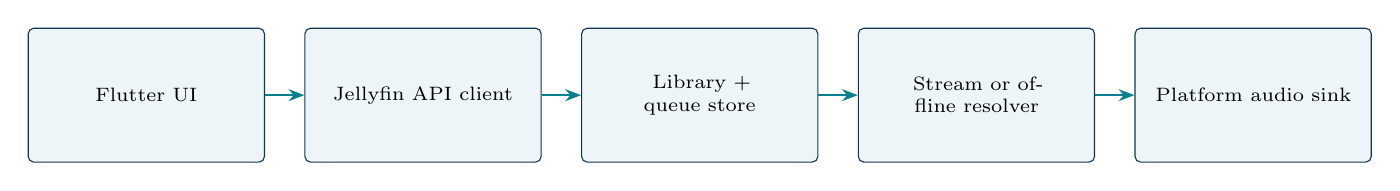
\begin{tikzpicture}[>=Stealth, node distance=1.4mm, every node/.style={font=\scriptsize,align=center}]
\node[draw=navy,rounded corners=2pt,fill=light,text width=26mm,minimum height=17mm,inner sep=2mm] (n0) {Flutter UI};
\node[draw=navy,rounded corners=2pt,fill=light,text width=26mm,minimum height=17mm,inner sep=2mm,right=5mm of n0] (n1) {Jellyfin API client};
\draw[-{Stealth[length=2mm]},thick,color=teal] (n0.east) -- (n1.west);
\node[draw=navy,rounded corners=2pt,fill=light,text width=26mm,minimum height=17mm,inner sep=2mm,right=5mm of n1] (n2) {Library + queue store};
\draw[-{Stealth[length=2mm]},thick,color=teal] (n1.east) -- (n2.west);
\node[draw=navy,rounded corners=2pt,fill=light,text width=26mm,minimum height=17mm,inner sep=2mm,right=5mm of n2] (n3) {Stream or offline resolver};
\draw[-{Stealth[length=2mm]},thick,color=teal] (n2.east) -- (n3.west);
\node[draw=navy,rounded corners=2pt,fill=light,text width=26mm,minimum height=17mm,inner sep=2mm,right=5mm of n3] (n4) {Platform audio sink};
\draw[-{Stealth[length=2mm]},thick,color=teal] (n3.east) -- (n4.west);
\end{tikzpicture}
\end{center}
\small\textit{Figure 7: Conceptual runtime path for a comparable implementation. This is not a traced source-code call graph.}\normalsize\par
\section{End-to-end user-to-speaker flow}
\begin{enumerate}[leftmargin=*,itemsep=2pt,topsep=2pt]
\item Client authenticates to a Jellyfin server and reads collection metadata.
\item Playback resolver checks for a complete validated local download.
\item Otherwise it requests direct or transcoded streaming based on settings and network.
\item Player emits progress, buffering and final listening events.
\item After reconnect, any pending offline listening records are reconciled to the server.
\end{enumerate}
\section{Data contract [P]}
\begin{evidencebox}\small\textbf{Candidate conceptual entities (not copied database classes):}\par
\begin{itemize}[leftmargin=*,itemsep=1pt,topsep=2pt]
\item \texttt{ServerAccount(base\_url, token\_ref, user\_id)}
\item \texttt{RemoteTrack(jellyfin\_id, codec, length)}
\item \texttt{OfflineManifest(item\_id, local\_path, checksum, status)}
\item \texttt{DownloadJob(id, retries, bytes\_total)}
\item \texttt{ListeningOutbox(item\_id, event, client\_time)}
\end{itemize}\end{evidencebox}
\section{Implementation blueprint [P]}
\begin{itemize}[leftmargin=*,itemsep=2pt,topsep=3pt]
\item Build an offline-first repository that resolves a single media item to verified local storage or an authorized remote URL.
\item Persist a manifest with download status, content version, checksum and resumable byte ranges where supported.
\item Keep a separate playback outbox for offline scrobbles; deduplicate idempotently on replay.
\item Model network/metered-data preferences; never silently substitute transcoded audio in a lossless mode.
\item Use one queue state source for Flutter views, lock-screen controls, Android Auto and CarPlay integrations.
\item Encrypt secrets in platform-protected storage and scope downloaded-file access to app sandbox.
\end{itemize}
\subsection*{Engineering equation}
\begin{equation*}\mathrm{Resolve}(m)=\begin{cases}\mathrm{local}(m),&\mathrm{complete}(m)\land\mathrm{verified}(m)\\\mathrm{remote}(m,q),&\mathrm{online}\land\mathrm{authorized}\\\mathrm{unavailable},&\mathrm{otherwise}\end{cases}\end{equation*}
Offline files take priority only when a complete and validated artifact is present; q captures stream/transcode quality choice.\par
\section{Validation and operational guardrails}
\textbf{Acceptance-test plan [P].}\par
\begin{itemize}[leftmargin=*,itemsep=2pt,topsep=3pt]
\item Airplane-mode tests, playback across reconnect, and partial-download recovery.
\item Duplicate scrobble prevention on retry and clock-skew tolerance.
\item Lossless-versus-transcoded display and gapless queue-transition tests.
\end{itemize}
\textbf{Constraints and risks [B].}\par
\begin{itemize}[leftmargin=*,itemsep=2pt,topsep=3pt]
\item No Jellyfin server means no indexed remote library.
\item Transcoding intentionally changes the media representation.
\item MPL-2.0 obligations and platform/plugin licences require component-by-component review.
\end{itemize}
\section*{Primary evidence and source entry points}
\begin{itemize}[leftmargin=*,itemsep=1pt,topsep=1pt]
\item \sourceurl{https://github.com/finamp-app/finamp}
\item \sourceurl{https://github.com/finamp-app/finamp/blob/redesign/README.md}
\end{itemize}
\clearpage
\section{UI/UX architecture and annotated screen concept}
\begin{evidencebox}\small\tagverified{} The official README provides redesigned screenshots of Home/Library, Now Playing, queue, downloads and lyrics; gapless audio, transcoding, offline downloads and dynamic colors are documented.\\[2pt]\textbf{UX evidence link:} \sourceurl{https://github.com/finamp-app/finamp}\\[2pt]\tagproposal{} The image, colors, exact screen compositions, flows, and acceptance criteria below are authored design recommendations, not release screenshots or audited internal UI components.\end{evidencebox}
\begin{center}
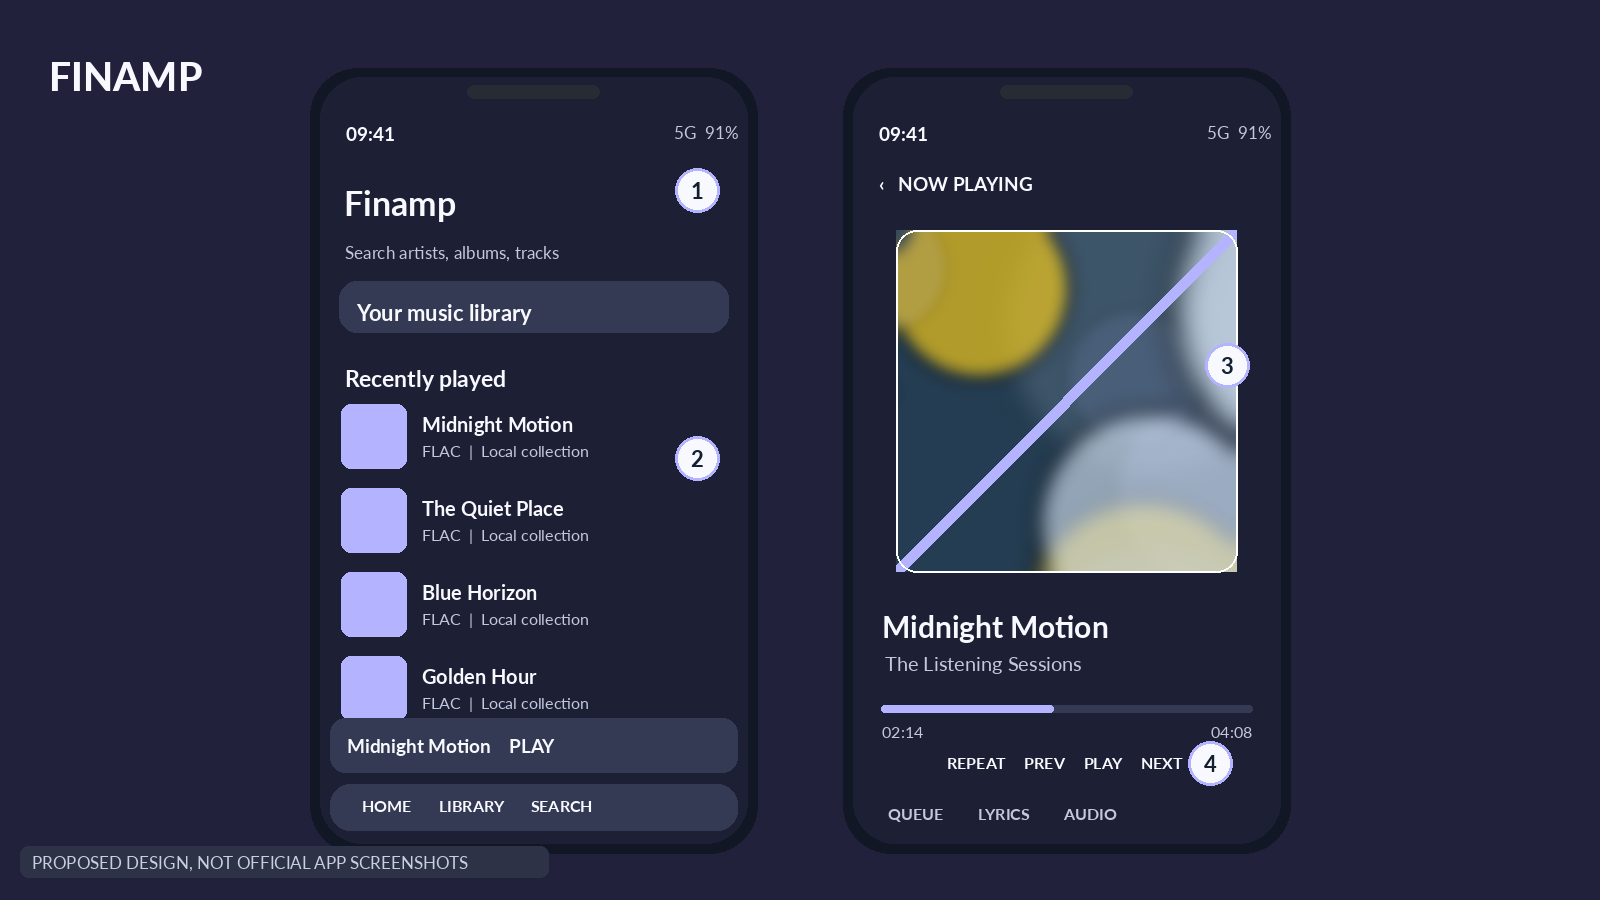
\includegraphics[width=\linewidth,height=93mm,keepaspectratio]{Music_Player_UIUX_Assets/finamp_concept.png}
\end{center}
{\small\color{muted}\textit{Annotated concept:} An adaptive personal-streaming client with strong offline reassurance: clear download status, server identity and playback quality. \textbf{Intended platform:} Flutter mobile + desktop. The visual uses invented album names and placeholder artwork.\par}
\subsection*{Proposed visual design system}
\begin{tabularx}{\linewidth}{@{}p{24mm}X@{}}
\textbf{Palette} & \colorbox[HTML]{1D2035}{\rule{6mm}{3mm}}\, Base 1D2035 \quad \colorbox[HTML]{B4B3FF}{\rule{6mm}{3mm}}\, Accent B4B3FF \\
\textbf{Typography} & Body 14--16 px; labels 12--13 px; primary screen heading 26--34 px; numeric audio data set in tabular figures.\\
\textbf{Spacing} & 4/8 px grid; 8--16 px card radius; align cover art to text blocks; 44 px touch-target minimum where relevant.\\
\textbf{Contrast} & Target WCAG AA text contrast, 4.5:1 for normal text and 3:1 for large text; verify final palette in both light/dark states.\\
\end{tabularx}
\subsection*{Annotated interface anatomy}
\begin{tabularx}{\linewidth}{@{}p{12mm}X@{}}\toprule Mark & Proposed region and responsibilities\\\midrule
\textbf{1} & Library navigation and recent music on primary mobile tab\\
\textbf{2} & Offline-ready track list with download badges in full prototype\\
\textbf{3} & Immersive cover art, adaptive colors and source identity\\
\textbf{4} & Player controls and reachable queue, lyrics, quality settings\\
\bottomrule\end{tabularx}
\clearpage
\section{UX functional specification [P]}
\subsection*{Information architecture and screens}
\begin{tabularx}{\linewidth}{@{}p{34mm}X@{}}\toprule Screen / route & Core content and controls\\\midrule
Server login & Jellyfin address, account selection and connectivity diagnosis\\
Home / Library & Albums, artists, latest, favorites and listening continuity\\
Now Playing & Album artwork, large transport, queue, lyrics and quality chip\\
Downloads & Queued/downloading/complete/failed states and offline storage budget\\
Streaming Settings & Direct versus transcode, mobile data policy, ReplayGain and device control\\
\bottomrule\end{tabularx}
\subsection*{Navigation model}
Thumb-friendly bottom navigation with a persistent mini-player; full-screen Now Playing as a vertical transition.\par
\subsection*{Critical user journeys}
\begin{enumerate}[leftmargin=*,itemsep=3pt,topsep=2pt]
\item \textbf{Go offline.} Select album; choose download quality; show task progress; open Downloads; play in airplane mode.
\item \textbf{Stream on mobile data.} Open quality chooser; inspect data estimate; choose transcode or original when offered.
\item \textbf{Resume interrupted download.} Re-enter network; auto-resume supported jobs; verify files; reconcile offline scrobble.
\end{enumerate}
\subsection*{Interaction, feedback and edge states}
Swipe queue reorder with alternative move menu, tap-to-seek, accessible offline actions, download progress announced semantically.\par
\begin{tabularx}{\linewidth}{@{}p{39mm}X@{}}\toprule State / trigger & Expected UX behavior\\\midrule
Server unreachable & Make offline library an immediately visible primary option.\\
Partial download & Clearly mark playable versus pending tracks; do not show as fully saved.\\
Network quality degraded & Show buffering/retry with chosen quality, not unannounced conversion.\\
\bottomrule\end{tabularx}
\subsection*{Implementation and QA contract}
\begin{itemize}[leftmargin=*,itemsep=2pt,topsep=2pt]
\item \textbf{Single source of truth.} Playback, queue and current destination/device belong to the application state model, not duplicated per view.
\item \textbf{Accessibility.} Keyboard navigation, screen-reader labels, visible focus, user-controlled lyric scrolling, reduced motion and non-color-only states.
\item \textbf{Responsive behavior.} Preserve transport when resizing; test narrow, zoomed and high-font settings; use alternative to drag-only controls.
\item \textbf{Instrumentation.} successful offline plays; failed download retry rate; reconnect recovery; data-mode change confidence.
\item \textbf{Boundary.} All remote content flows through a separately configured Jellyfin server; do not promise standalone library ingestion.
\end{itemize}
\vspace{2mm}\begin{evidencebox}\small\textbf{Prototype acceptance:} Primary play and pause remain available through every screen; the queue and playback position survive navigation; every error has recovery text; every advertised fidelity setting accurately reflects the active engine/device. Design specifications are recommendations and require product usability testing.\end{evidencebox}
\clearpage
\chapter{Gramophone}
{\large\color{muted}Media3-based Android player with Material 3 design}\par
\begin{evidencebox}\small\textbf{Repository:} \sourceurl{https://github.com/FoedusProgramme/Gramophone}\\\textbf{Reference branch:} beta\qquad \textbf{License:} GPL-3.0\\\textbf{Primary stack:} Android/Kotlin app; Media3; Material Design UI; Android MediaStore; custom hificore module.\end{evidencebox}
\section{Observed system architecture [V]}
\begin{itemize}[leftmargin=*,itemsep=2pt,topsep=3pt]
\item README states use of Media3 and Material Design, plus MediaStore-based local indexing.
\item UI features include dynamic Monet color, playlist/folder browse and word-level synchronized lyrics.
\item Repository contains a hificore directory and Media3 git submodule; build notes require recursive submodule checkout.
\end{itemize}
\textbf{Visible source anchors [V].} app/, hificore/, media3 submodule, baselineprofile/, settings.gradle.kts, build.gradle.kts.\par
\begin{evidencebox}\tagboundary{} The exact hificore native signal path has not been reconstructed; no unsupported exclusive-mode or bit-perfect capability is attributed to the project.\end{evidencebox}
\section{Functional block blueprint [P]}
\begin{center}
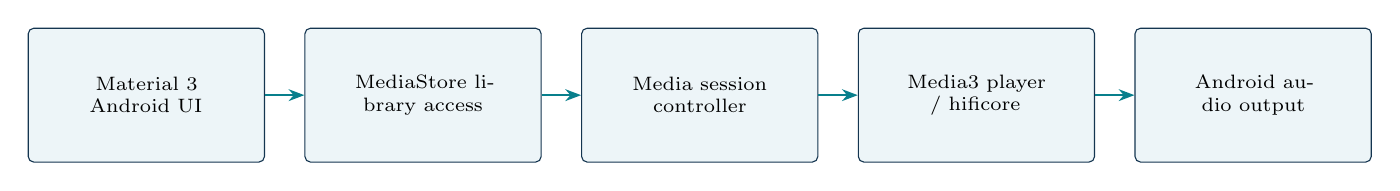
\begin{tikzpicture}[>=Stealth, node distance=1.4mm, every node/.style={font=\scriptsize,align=center}]
\node[draw=navy,rounded corners=2pt,fill=light,text width=26mm,minimum height=17mm,inner sep=2mm] (n0) {Material 3 Android UI};
\node[draw=navy,rounded corners=2pt,fill=light,text width=26mm,minimum height=17mm,inner sep=2mm,right=5mm of n0] (n1) {MediaStore library access};
\draw[-{Stealth[length=2mm]},thick,color=teal] (n0.east) -- (n1.west);
\node[draw=navy,rounded corners=2pt,fill=light,text width=26mm,minimum height=17mm,inner sep=2mm,right=5mm of n1] (n2) {Media session controller};
\draw[-{Stealth[length=2mm]},thick,color=teal] (n1.east) -- (n2.west);
\node[draw=navy,rounded corners=2pt,fill=light,text width=26mm,minimum height=17mm,inner sep=2mm,right=5mm of n2] (n3) {Media3 player / hificore};
\draw[-{Stealth[length=2mm]},thick,color=teal] (n2.east) -- (n3.west);
\node[draw=navy,rounded corners=2pt,fill=light,text width=26mm,minimum height=17mm,inner sep=2mm,right=5mm of n3] (n4) {Android audio output};
\draw[-{Stealth[length=2mm]},thick,color=teal] (n3.east) -- (n4.west);
\end{tikzpicture}
\end{center}
\small\textit{Figure 8: Conceptual runtime path for a comparable implementation. This is not a traced source-code call graph.}\normalsize\par
\section{End-to-end user-to-speaker flow}
\begin{enumerate}[leftmargin=*,itemsep=2pt,topsep=2pt]
\item Android grants the scoped audio-library permission.
\item MediaStore query builds track and folder views.
\item User selects a track; media session and Media3 player load its content URI.
\item Playback status and metadata inform notifications and external transport controls.
\item Timed lyric parser updates word- or syllable-level highlighted text.
\end{enumerate}
\section{Data contract [P]}
\begin{evidencebox}\small\textbf{Candidate conceptual entities (not copied database classes):}\par
\begin{itemize}[leftmargin=*,itemsep=1pt,topsep=2pt]
\item \texttt{MediaStoreTrack(content\_uri, media\_id, tags)}
\item \texttt{Playlist(id, entries)}
\item \texttt{PlayerSession(queue, index, position)}
\item \texttt{LyricCue(timestamp, word\_offset, text)}
\item \texttt{GainSettings(enabled, source\_tag)}
\end{itemize}\end{evidencebox}
\section{Implementation blueprint [P]}
\begin{itemize}[leftmargin=*,itemsep=2pt,topsep=3pt]
\item Follow scoped storage: use content URIs instead of raw unrestricted paths.
\item Treat Media3 SessionService and controller as the playback contract for foreground/background UI.
\item Keep a MediaRepository and LyricsRepository separate from activity/fragment rendering.
\item Cache parsed LRC/TTML/SRT word timing with versioned parsing to avoid work on every frame.
\item Offer ReplayGain toggles with clearly documented source tag behavior.
\item Run baseline profile/performance builds and preserve Play Store/F-Droid signing distinctions.
\end{itemize}
\subsection*{Engineering equation}
\begin{equation*}k(t)=\max\{i:\tau_i\le t\},\qquad \mathrm{LyricHighlight}(t)=\mathrm{token}_{k(t)}\end{equation*}
The active lyric token is the most recent cue at or before playback time; seek must update the index immediately.\par
\section{Validation and operational guardrails}
\textbf{Acceptance-test plan [P].}\par
\begin{itemize}[leftmargin=*,itemsep=2pt,topsep=3pt]
\item MediaStore permission and revoked-access tests.
\item Lyrics parsing golden tests for LRC, TTML and SRT; rapid seeking.
\item Media session and notification controls while app UI is closed.
\end{itemize}
\textbf{Constraints and risks [B].}\par
\begin{itemize}[leftmargin=*,itemsep=2pt,topsep=3pt]
\item Android codec availability varies by OS version and device.
\item Patched or submodule Media3 builds need strict dependency pinning.
\item GPL-3.0 applies to redistributed modifications.
\end{itemize}
\section*{Primary evidence and source entry points}
\begin{itemize}[leftmargin=*,itemsep=1pt,topsep=1pt]
\item \sourceurl{https://github.com/FoedusProgramme/Gramophone}
\item \sourceurl{https://github.com/FoedusProgramme/Gramophone/blob/beta/readme.md}
\end{itemize}
\clearpage
\section{UI/UX architecture and annotated screen concept}
\begin{evidencebox}\small\tagverified{} The README documents Material 3, dynamic Monet colors, MediaStore browsing, folder views, playlists, ReplayGain 2.0 and synchronized LRC/TTML/SRT lyrics including word-level highlighting.\\[2pt]\textbf{UX evidence link:} \sourceurl{https://github.com/FoedusProgramme/Gramophone}\\[2pt]\tagproposal{} The image, colors, exact screen compositions, flows, and acceptance criteria below are authored design recommendations, not release screenshots or audited internal UI components.\end{evidencebox}
\begin{center}
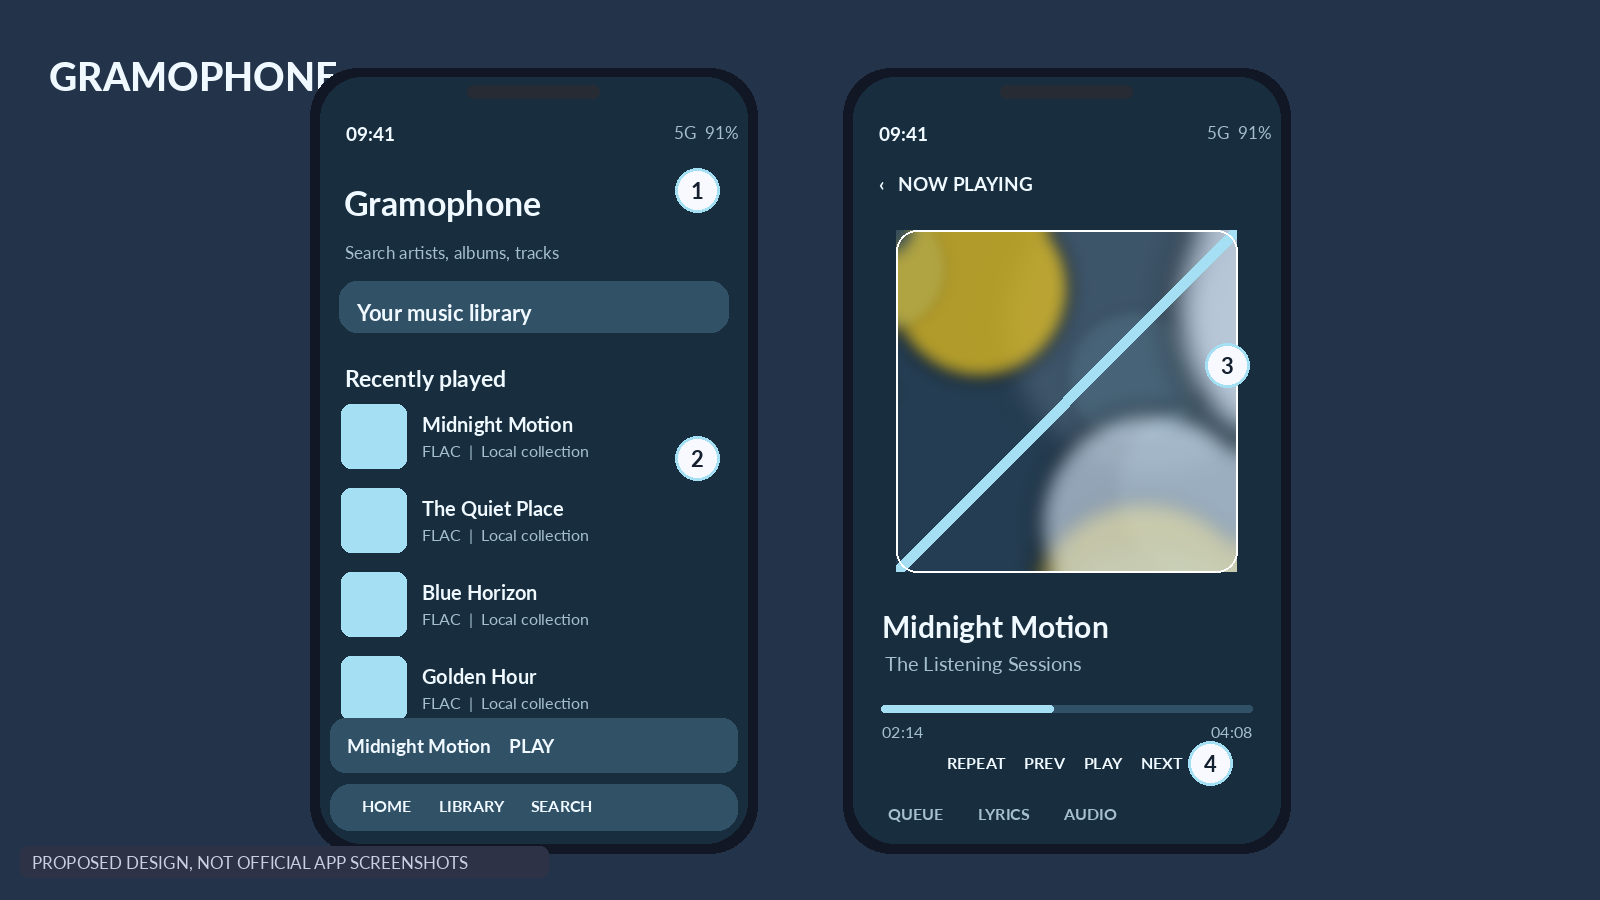
\includegraphics[width=\linewidth,height=93mm,keepaspectratio]{Music_Player_UIUX_Assets/gramophone_concept.png}
\end{center}
{\small\color{muted}\textit{Annotated concept:} Material You correctness first: adaptive surface colors, robust dark/light contrast, predictable motion and system-integrated media controls. \textbf{Intended platform:} Native Android. The visual uses invented album names and placeholder artwork.\par}
\subsection*{Proposed visual design system}
\begin{tabularx}{\linewidth}{@{}p{24mm}X@{}}
\textbf{Palette} & \colorbox[HTML]{182E3E}{\rule{6mm}{3mm}}\, Base 182E3E \quad \colorbox[HTML]{A5DFF3}{\rule{6mm}{3mm}}\, Accent A5DFF3 \\
\textbf{Typography} & Body 14--16 px; labels 12--13 px; primary screen heading 26--34 px; numeric audio data set in tabular figures.\\
\textbf{Spacing} & 4/8 px grid; 8--16 px card radius; align cover art to text blocks; 44 px touch-target minimum where relevant.\\
\textbf{Contrast} & Target WCAG AA text contrast, 4.5:1 for normal text and 3:1 for large text; verify final palette in both light/dark states.\\
\end{tabularx}
\subsection*{Annotated interface anatomy}
\begin{tabularx}{\linewidth}{@{}p{12mm}X@{}}\toprule Mark & Proposed region and responsibilities\\\midrule
\textbf{1} & Material 3 library taxonomy and search entry\\
\textbf{2} & Album and song list with type-scalable rows\\
\textbf{3} & Artwork-driven now-playing and lyric entry point\\
\textbf{4} & Android playback buttons with Media3 session parity\\
\bottomrule\end{tabularx}
\clearpage
\section{UX functional specification [P]}
\subsection*{Information architecture and screens}
\begin{tabularx}{\linewidth}{@{}p{34mm}X@{}}\toprule Screen / route & Core content and controls\\\midrule
Library / Browse & Tracks, albums, artists, folders and sort menus\\
Album detail & Palette-derived artwork header and reliable track list\\
Now Playing & Artwork, lyrics and transport with Android Media3 controls\\
Synced Lyrics & Time-coded line and word highlight, no forced auto-scroll for manual readers\\
Playback Settings & ReplayGain, system EQ handoff, format disclosures and UI preferences\\
\bottomrule\end{tabularx}
\subsection*{Navigation model}
Material navigation components with an anchored mini-player; immersive album/lyrics screens follow system back stack.\par
\subsection*{Critical user journeys}
\begin{enumerate}[leftmargin=*,itemsep=3pt,topsep=2pt]
\item \textbf{Grant media permission.} Explain on-device audio scope; request runtime permission; load MediaStore.
\item \textbf{Browse to song.} Open album; tap track; expand mini-player; inspect synced lyrics.
\item \textbf{Hand off to system.} Use headset controls, notification and lock screen; preserve one queue owner.
\end{enumerate}
\subsection*{Interaction, feedback and edge states}
Predictive back, haptic feedback sparingly, large tap targets and support for accessibility font scaling without artwork overlap.\par
\begin{tabularx}{\linewidth}{@{}p{39mm}X@{}}\toprule State / trigger & Expected UX behavior\\\midrule
MediaStore empty & Explain permission versus truly empty library; offer folder guidance.\\
Lyrics desynchronized & Offer offset adjustment without altering underlying file.\\
No equalizer activity & Explain third-party equalizer support and Android permission boundaries.\\
\bottomrule\end{tabularx}
\subsection*{Implementation and QA contract}
\begin{itemize}[leftmargin=*,itemsep=2pt,topsep=2pt]
\item \textbf{Single source of truth.} Playback, queue and current destination/device belong to the application state model, not duplicated per view.
\item \textbf{Accessibility.} Keyboard navigation, screen-reader labels, visible focus, user-controlled lyric scrolling, reduced motion and non-color-only states.
\item \textbf{Responsive behavior.} Preserve transport when resizing; test narrow, zoomed and high-font settings; use alternative to drag-only controls.
\item \textbf{Instrumentation.} permission-to-library conversion; time to now playing; lyric timing correction rate; service resurrection after OS eviction.
\item \textbf{Boundary.} Do not claim unsupported device-level exclusive/bit-perfect audio merely because hificore or Media3 modules exist.
\end{itemize}
\vspace{2mm}\begin{evidencebox}\small\textbf{Prototype acceptance:} Primary play and pause remain available through every screen; the queue and playback position survive navigation; every error has recovery text; every advertised fidelity setting accurately reflects the active engine/device. Design specifications are recommendations and require product usability testing.\end{evidencebox}
\clearpage
\chapter{Auxio}
{\large\color{muted}Privacy-first offline Android player with custom metadata layer}\par
\begin{evidencebox}\small\textbf{Repository:} \sourceurl{https://github.com/OxygenCobalt/Auxio}\\\textbf{Reference branch:} dev\qquad \textbf{License:} GPL-3.0-or-later\\\textbf{Primary stack:} Android/Kotlin; Media3 ExoPlayer with project-specific patches; native media index and TagLib metadata integration.\end{evidencebox}
\section{Observed system architecture [V]}
\begin{itemize}[leftmargin=*,itemsep=2pt,topsep=3pt]
\item README names Media3 ExoPlayer, a patched Media3 version, and TagLib for metadata parsing.
\item Features include gapless playback, ReplayGain, artist/album-artist logic, detailed tags and Android Auto.
\item Explicitly local, offline and privacy-focused; supports local storage and SD-card-aware folder access.
\end{itemize}
\textbf{Visible source anchors [V].} app/, musikr/, media submodule, build.gradle, settings.gradle, README.md.\par
\begin{evidencebox}\tagboundary{} The index shape and Kotlin domain interfaces below are proposed abstractions; exact implementation classes were not verified line-by-line.\end{evidencebox}
\section{Functional block blueprint [P]}
\begin{center}
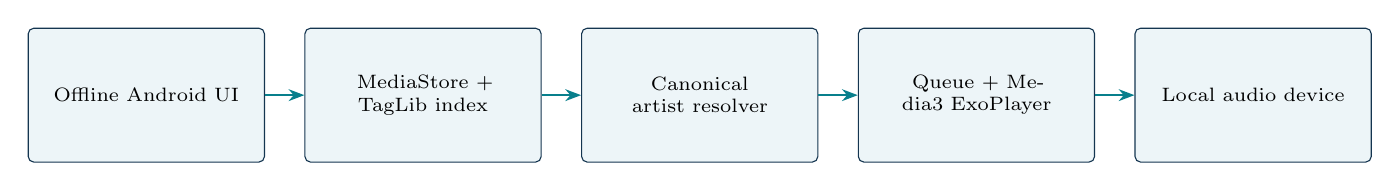
\begin{tikzpicture}[>=Stealth, node distance=1.4mm, every node/.style={font=\scriptsize,align=center}]
\node[draw=navy,rounded corners=2pt,fill=light,text width=26mm,minimum height=17mm,inner sep=2mm] (n0) {Offline Android UI};
\node[draw=navy,rounded corners=2pt,fill=light,text width=26mm,minimum height=17mm,inner sep=2mm,right=5mm of n0] (n1) {MediaStore + TagLib index};
\draw[-{Stealth[length=2mm]},thick,color=teal] (n0.east) -- (n1.west);
\node[draw=navy,rounded corners=2pt,fill=light,text width=26mm,minimum height=17mm,inner sep=2mm,right=5mm of n1] (n2) {Canonical artist resolver};
\draw[-{Stealth[length=2mm]},thick,color=teal] (n1.east) -- (n2.west);
\node[draw=navy,rounded corners=2pt,fill=light,text width=26mm,minimum height=17mm,inner sep=2mm,right=5mm of n2] (n3) {Queue + Media3 ExoPlayer};
\draw[-{Stealth[length=2mm]},thick,color=teal] (n2.east) -- (n3.west);
\node[draw=navy,rounded corners=2pt,fill=light,text width=26mm,minimum height=17mm,inner sep=2mm,right=5mm of n3] (n4) {Local audio device};
\draw[-{Stealth[length=2mm]},thick,color=teal] (n3.east) -- (n4.west);
\end{tikzpicture}
\end{center}
\small\textit{Figure 9: Conceptual runtime path for a comparable implementation. This is not a traced source-code call graph.}\normalsize\par
\section{End-to-end user-to-speaker flow}
\begin{enumerate}[leftmargin=*,itemsep=2pt,topsep=2pt]
\item User grants local audio-library access.
\item Indexer reads MediaStore data and detailed file tags via TagLib.
\item Metadata normalization computes artist/album-artist groupings.
\item Queue persists track identifiers and position.
\item Media3 ExoPlayer handles local gapless playback, ReplayGain and media-session controls.
\end{enumerate}
\section{Data contract [P]}
\begin{evidencebox}\small\textbf{Candidate conceptual entities (not copied database classes):}\par
\begin{itemize}[leftmargin=*,itemsep=1pt,topsep=2pt]
\item \texttt{Song(uri, disc, track, release\_date)}
\item \texttt{Artist(id, display\_name, source\_tags)}
\item \texttt{ArtistAlias(alias, canonical\_artist\_id)}
\item \texttt{AlbumArtistLink(album\_id, artist\_id)}
\item \texttt{PlaybackBookmark(queue\_id, index, offset\_ms)}
\end{itemize}\end{evidencebox}
\section{Implementation blueprint [P]}
\begin{itemize}[leftmargin=*,itemsep=2pt,topsep=3pt]
\item Normalize tags into stable artist and album-artist entities, preserving raw source tags for debugging.
\item Separate background metadata parsing from UI so large scans never block scrolling.
\item Use a content-URI resolver robust to SD card removal and metadata renames.
\item Persist an atomic queue snapshot with resume index/offset and validate entries on restore.
\item Keep Media3 patches documented, upstream-diffed and covered by regression tests.
\item Avoid telemetry or network permission unless user explicitly enables a future optional integration.
\end{itemize}
\subsection*{Engineering equation}
\begin{equation*}\mathrm{ArtistKey}=H(\mathrm{normalized\ name},\mathrm{album\ artist\ scope})\end{equation*}
A suggested canonicalization approach; identity must be reconciled with aliases, stable IDs and source metadata to avoid collisions.\par
\section{Validation and operational guardrails}
\textbf{Acceptance-test plan [P].}\par
\begin{itemize}[leftmargin=*,itemsep=2pt,topsep=3pt]
\item Multi-artist and album-artist golden data fixtures.
\item Unmount/re-mount SD card and revoked-permission robustness.
\item ReplayGain, gapless, Android Auto and queue persistence tests.
\end{itemize}
\textbf{Constraints and risks [B].}\par
\begin{itemize}[leftmargin=*,itemsep=2pt,topsep=3pt]
\item Patched Media3 raises merge/rebase maintenance cost.
\item Android device output still determines achievable Hi-Fi mode.
\item GPL-3.0-or-later obligations apply to forks.
\end{itemize}
\section*{Primary evidence and source entry points}
\begin{itemize}[leftmargin=*,itemsep=1pt,topsep=1pt]
\item \sourceurl{https://github.com/OxygenCobalt/Auxio}
\item \sourceurl{https://github.com/OxygenCobalt/Auxio/blob/dev/README.md}
\end{itemize}
\clearpage
\section{UI/UX architecture and annotated screen concept}
\begin{evidencebox}\small\tagverified{} The README documents Media3 ExoPlayer, advanced tags, folder/SD card support, playlists, gapless, ReplayGain, widgets, search, Android Auto and an offline/private design.\\[2pt]\textbf{UX evidence link:} \sourceurl{https://github.com/OxygenCobalt/Auxio}\\[2pt]\tagproposal{} The image, colors, exact screen compositions, flows, and acceptance criteria below are authored design recommendations, not release screenshots or audited internal UI components.\end{evidencebox}
\begin{center}
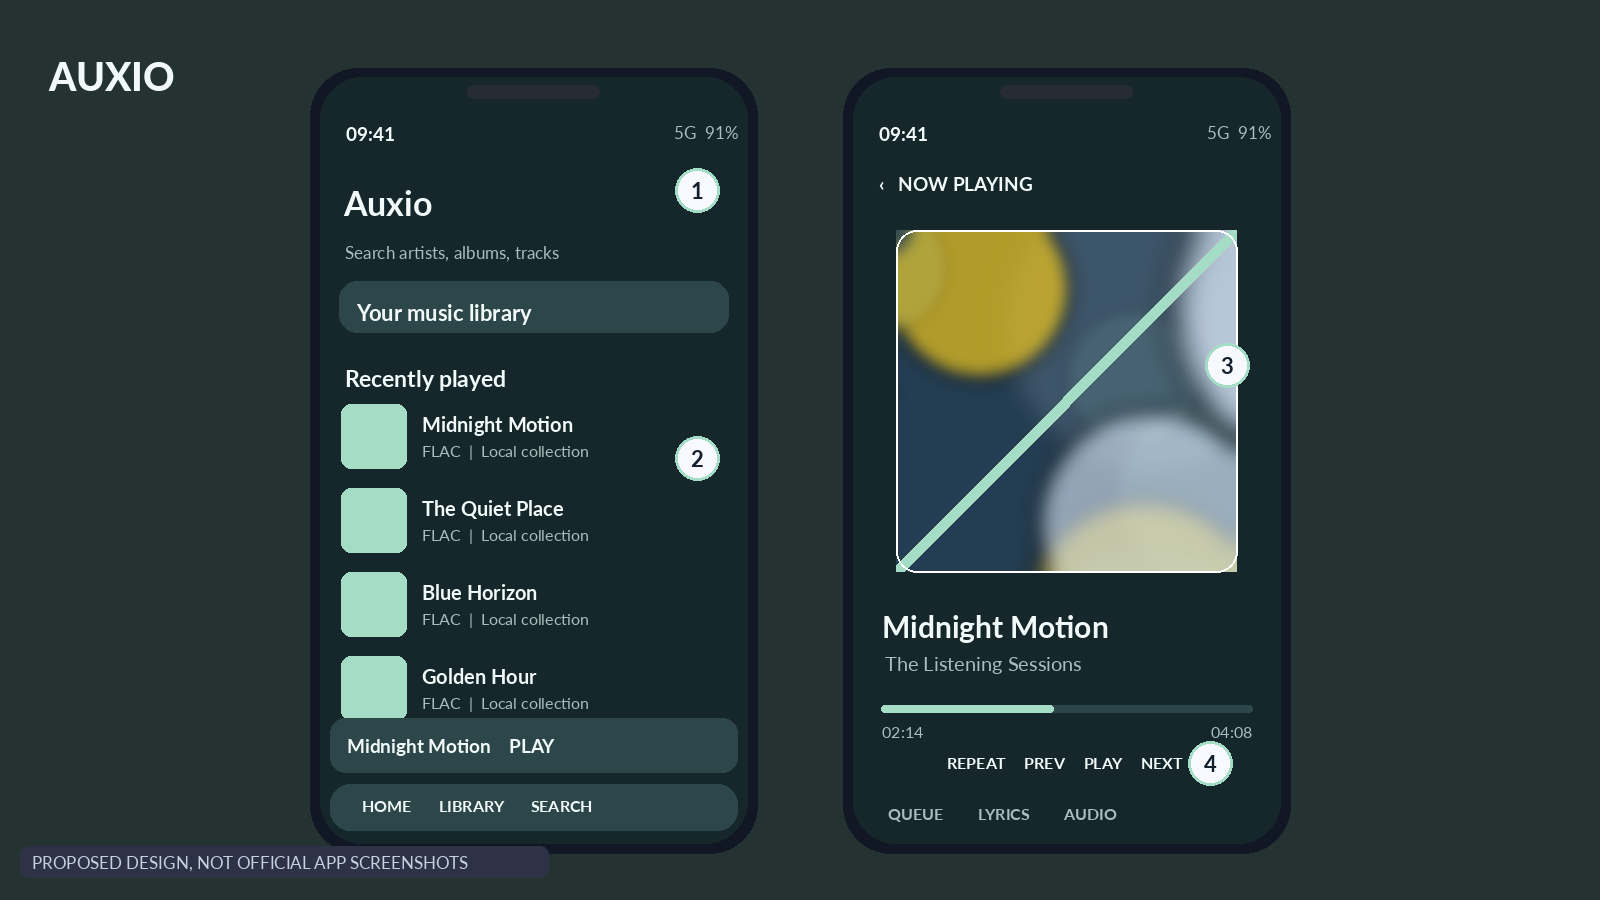
\includegraphics[width=\linewidth,height=93mm,keepaspectratio]{Music_Player_UIUX_Assets/auxio_concept.png}
\end{center}
{\small\color{muted}\textit{Annotated concept:} Utility with intent: highly legible lists, strong metadata fidelity, strict offline privacy and rapid navigation. \textbf{Intended platform:} Native offline Android. The visual uses invented album names and placeholder artwork.\par}
\subsection*{Proposed visual design system}
\begin{tabularx}{\linewidth}{@{}p{24mm}X@{}}
\textbf{Palette} & \colorbox[HTML]{15272B}{\rule{6mm}{3mm}}\, Base 15272B \quad \colorbox[HTML]{A4DCC6}{\rule{6mm}{3mm}}\, Accent A4DCC6 \\
\textbf{Typography} & Body 14--16 px; labels 12--13 px; primary screen heading 26--34 px; numeric audio data set in tabular figures.\\
\textbf{Spacing} & 4/8 px grid; 8--16 px card radius; align cover art to text blocks; 44 px touch-target minimum where relevant.\\
\textbf{Contrast} & Target WCAG AA text contrast, 4.5:1 for normal text and 3:1 for large text; verify final palette in both light/dark states.\\
\end{tabularx}
\subsection*{Annotated interface anatomy}
\begin{tabularx}{\linewidth}{@{}p{12mm}X@{}}\toprule Mark & Proposed region and responsibilities\\\midrule
\textbf{1} & Fast offline library and local search\\
\textbf{2} & Clear on-device file and advanced-tag handling\\
\textbf{3} & Focused artwork and track identity; no remote-library dependency\\
\textbf{4} & Gapless/ReplayGain state and foreground transport controls\\
\bottomrule\end{tabularx}
\clearpage
\section{UX functional specification [P]}
\subsection*{Information architecture and screens}
\begin{tabularx}{\linewidth}{@{}p{34mm}X@{}}\toprule Screen / route & Core content and controls\\\midrule
All Music & Songs, albums, artist and genre filters with fast scrolling\\
Folder / SD-card & Storage roots and transparent missing-card behavior\\
Search & Instant local matches, recent query memory optional\\
Now Playing + Queue & Gapless playback, ReplayGain disclosure and ordering\\
Settings / Privacy & Offline statement, permissions, metadata interpretation and advanced rules\\
\bottomrule\end{tabularx}
\subsection*{Navigation model}
Short bottom-level navigation + sortable listing; minimize modal layers; preserve the player while switching tabs.\par
\subsection*{Critical user journeys}
\begin{enumerate}[leftmargin=*,itemsep=3pt,topsep=2pt]
\item \textbf{Load on-device songs.} Grant access; scan MediaStore and tags; reconcile artist/album artist identities.
\item \textbf{Search offline.} Type search; tap result; play immediately; do not require network.
\item \textbf{Remove SD card.} Detect missing root; maintain safe stale entries; restore cleanly when remounted.
\end{enumerate}
\subsection*{Interaction, feedback and edge states}
Single tap play; long press contextual actions; accessibility node names include song, artist and duration; compact widgets.\par
\begin{tabularx}{\linewidth}{@{}p{39mm}X@{}}\toprule State / trigger & Expected UX behavior\\\midrule
Storage removable & Mark unavailable tracks, never erase user playlists automatically.\\
Metadata mismatch & Allow tag inspection with human-readable source and fallback.\\
No network & Work normally; avoid connectivity banners and nonessential online services.\\
\bottomrule\end{tabularx}
\subsection*{Implementation and QA contract}
\begin{itemize}[leftmargin=*,itemsep=2pt,topsep=2pt]
\item \textbf{Single source of truth.} Playback, queue and current destination/device belong to the application state model, not duplicated per view.
\item \textbf{Accessibility.} Keyboard navigation, screen-reader labels, visible focus, user-controlled lyric scrolling, reduced motion and non-color-only states.
\item \textbf{Responsive behavior.} Preserve transport when resizing; test narrow, zoomed and high-font settings; use alternative to drag-only controls.
\item \textbf{Instrumentation.} local search response; SD card recoverability; headset actions; playlist persistence; screen-reader route completion.
\item \textbf{Boundary.} The patched Media3 and taglib build dependencies need careful auditing, especially for redistributed variants.
\end{itemize}
\vspace{2mm}\begin{evidencebox}\small\textbf{Prototype acceptance:} Primary play and pause remain available through every screen; the queue and playback position survive navigation; every error has recovery text; every advertised fidelity setting accurately reflects the active engine/device. Design specifications are recommendations and require product usability testing.\end{evidencebox}
\clearpage
\chapter{Retro Music Player}
{\large\color{muted}Visual-theme-focused local Android music player}\par
\begin{evidencebox}\small\textbf{Repository:} \sourceurl{https://github.com/RetroMusicPlayer/RetroMusicPlayer}\\\textbf{Reference branch:} dev\qquad \textbf{License:} GPL-3.0\\\textbf{Primary stack:} Android/Kotlin; Material You/theming; local MediaStore; app and appthemehelper Gradle modules.\end{evidencebox}
\section{Observed system architecture [V]}
\begin{itemize}[leftmargin=*,itemsep=2pt,topsep=3pt]
\item Official README states this is a local Android music player, not an online downloader or streaming service.
\item Repository includes app and appthemehelper modules, screenshots and Gradle setup.
\item Project advertises multiple visual themes, widgets, playlists, folder navigation and now-playing customization.
\end{itemize}
\textbf{Visible source anchors [V].} app/, appthemehelper/, fastlane/, screenshots/, build.gradle.kts, LICENSE.md.\par
\begin{evidencebox}\tagboundary{} Repository topics mention MVVM and Koin, but exact present-day dependency wiring was not audited; view-model boundaries below are reference architecture.\end{evidencebox}
\section{Functional block blueprint [P]}
\begin{center}
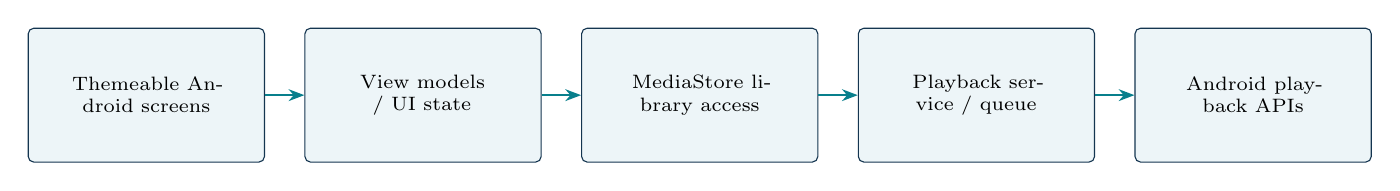
\begin{tikzpicture}[>=Stealth, node distance=1.4mm, every node/.style={font=\scriptsize,align=center}]
\node[draw=navy,rounded corners=2pt,fill=light,text width=26mm,minimum height=17mm,inner sep=2mm] (n0) {Themeable Android screens};
\node[draw=navy,rounded corners=2pt,fill=light,text width=26mm,minimum height=17mm,inner sep=2mm,right=5mm of n0] (n1) {View models / UI state};
\draw[-{Stealth[length=2mm]},thick,color=teal] (n0.east) -- (n1.west);
\node[draw=navy,rounded corners=2pt,fill=light,text width=26mm,minimum height=17mm,inner sep=2mm,right=5mm of n1] (n2) {MediaStore library access};
\draw[-{Stealth[length=2mm]},thick,color=teal] (n1.east) -- (n2.west);
\node[draw=navy,rounded corners=2pt,fill=light,text width=26mm,minimum height=17mm,inner sep=2mm,right=5mm of n2] (n3) {Playback service / queue};
\draw[-{Stealth[length=2mm]},thick,color=teal] (n2.east) -- (n3.west);
\node[draw=navy,rounded corners=2pt,fill=light,text width=26mm,minimum height=17mm,inner sep=2mm,right=5mm of n3] (n4) {Android playback APIs};
\draw[-{Stealth[length=2mm]},thick,color=teal] (n3.east) -- (n4.west);
\end{tikzpicture}
\end{center}
\small\textit{Figure 10: Conceptual runtime path for a comparable implementation. This is not a traced source-code call graph.}\normalsize\par
\section{End-to-end user-to-speaker flow}
\begin{enumerate}[leftmargin=*,itemsep=2pt,topsep=2pt]
\item User selects local songs or playlist from MediaStore-backed catalog.
\item UI resolves theme tokens, active now-playing style and artwork colors.
\item Playback state transitions update mini-player and expanded now-playing view.
\item Background playback integrates with Android notifications and headset controls.
\item Theme and queue preferences persist between app sessions.
\end{enumerate}
\section{Data contract [P]}
\begin{evidencebox}\small\textbf{Candidate conceptual entities (not copied database classes):}\par
\begin{itemize}[leftmargin=*,itemsep=1pt,topsep=2pt]
\item \texttt{ThemePreset(id, palette, typography, layout)}
\item \texttt{Song(uri, title, album\_art\_uri)}
\item \texttt{Playlist(id, entries)}
\item \texttt{NowPlayingLayout(id, artwork\_mode)}
\item \texttt{PlaybackOptions(repeat, shuffle, equalizer\_target)}
\end{itemize}\end{evidencebox}
\section{Implementation blueprint [P]}
\begin{itemize}[leftmargin=*,itemsep=2pt,topsep=3pt]
\item Treat appearance as a product subsystem: tokens for typography, spacing, colors, elevations and artwork effects.
\item Do not couple music library domain logic to one now-playing layout; render from a single immutable player state.
\item Use a MediaRepository boundary for local browse/search and a PlaybackFacade for queue controls.
\item Precompute artwork colors and thumbnails away from the main thread.
\item Provide accessible contrast modes, reduced motion and predictable player controls.
\item Keep future streaming support as an optional new provider; do not misrepresent it as a current capability.
\end{itemize}
\subsection*{Engineering equation}
\begin{equation*}C_{\mathrm{text}}\ge 4.5:1\quad\text{(target for normal-sized text)}\end{equation*}
A recommended contrast target for premium themes, not an assertion that every Retro Music Player theme passes accessibility audits.\par
\section{Validation and operational guardrails}
\textbf{Acceptance-test plan [P].}\par
\begin{itemize}[leftmargin=*,itemsep=2pt,topsep=3pt]
\item Screenshot regression matrix across dark/light, dynamic color and compact layouts.
\item Scroll-performance tests with large libraries and oversized album artwork.
\item MediaStore and background notification playback compatibility tests.
\end{itemize}
\textbf{Constraints and risks [B].}\par
\begin{itemize}[leftmargin=*,itemsep=2pt,topsep=3pt]
\item UI quality can degrade quickly if theme logic is scattered across screens.
\item No native online streaming capability is claimed by the official project.
\item GPL-3.0 limits redistribution as a proprietary rebrand.
\end{itemize}
\section*{Primary evidence and source entry points}
\begin{itemize}[leftmargin=*,itemsep=1pt,topsep=1pt]
\item \sourceurl{https://github.com/RetroMusicPlayer/RetroMusicPlayer}
\item \sourceurl{https://retromusic.app/RetroMusicPlayer}
\item \sourceurl{https://github.com/RetroMusicPlayer/RetroMusicPlayer/blob/dev/README.md}
\end{itemize}
\clearpage
\section{UI/UX architecture and annotated screen concept}
\begin{evidencebox}\small\tagverified{} The official site documents Clearly White, Kinda Dark and Just Black themes, configurable navigation, many Now Playing designs, lyrics, widgets, and an entirely local playback model.\\[2pt]\textbf{UX evidence link:} \sourceurl{https://retromusic.app/}\\[2pt]\tagproposal{} The image, colors, exact screen compositions, flows, and acceptance criteria below are authored design recommendations, not release screenshots or audited internal UI components.\end{evidencebox}
\begin{center}
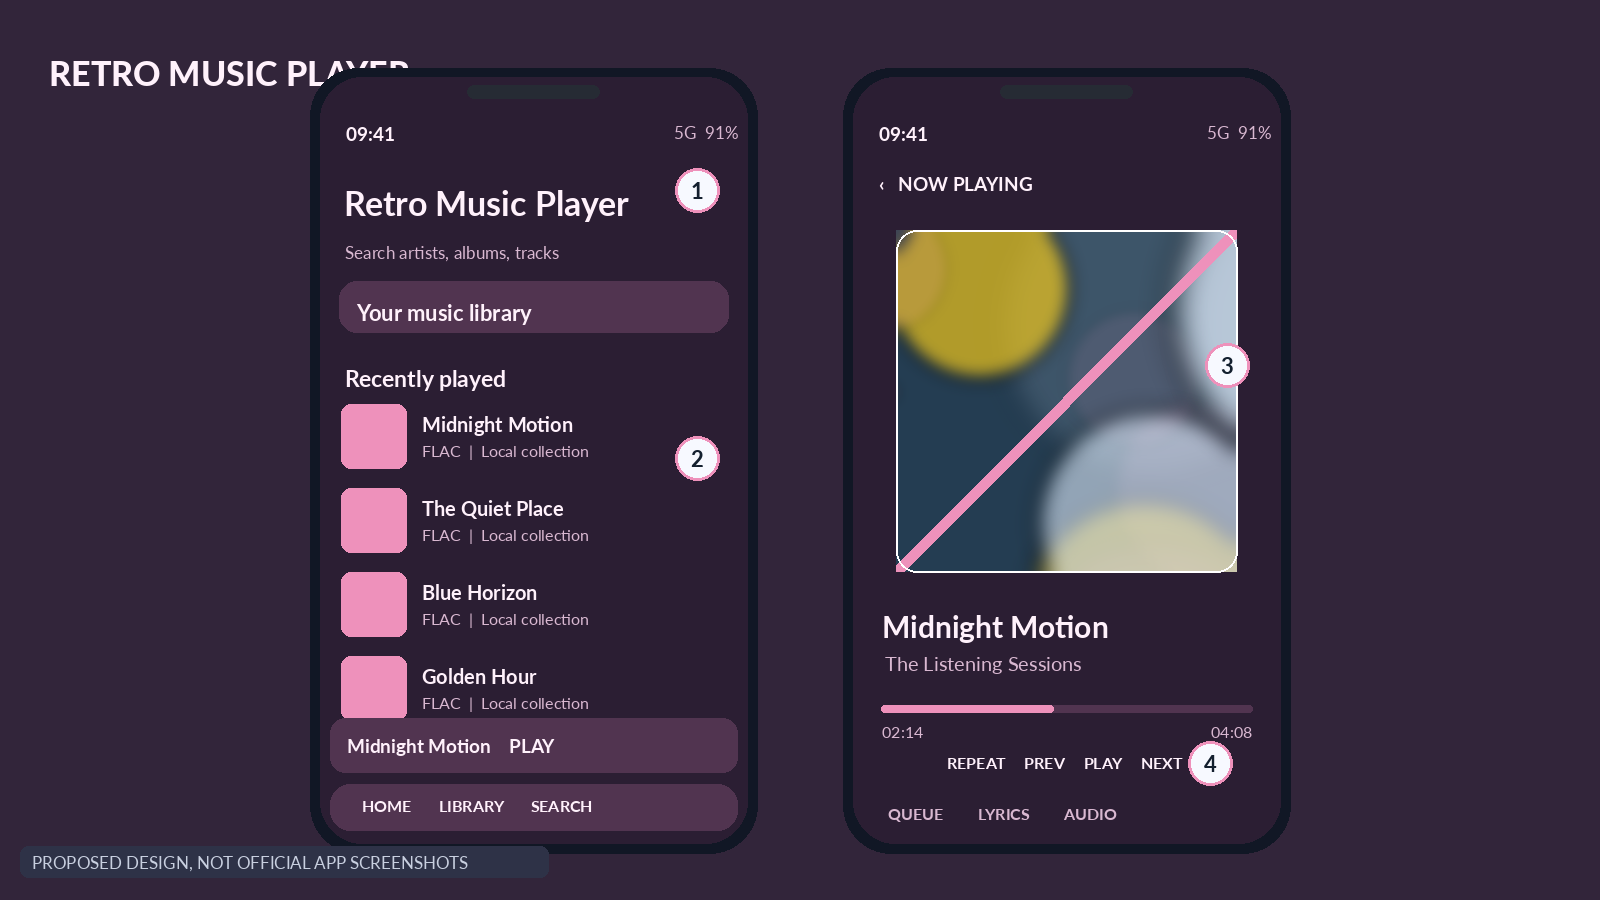
\includegraphics[width=\linewidth,height=93mm,keepaspectratio]{Music_Player_UIUX_Assets/retro_music_player_concept.png}
\end{center}
{\small\color{muted}\textit{Annotated concept:} A richly customizable visual identity with bold cover gradients, theme presets and discoverable personalization without sacrificing playback usability. \textbf{Intended platform:} Native offline Android. The visual uses invented album names and placeholder artwork.\par}
\subsection*{Proposed visual design system}
\begin{tabularx}{\linewidth}{@{}p{24mm}X@{}}
\textbf{Palette} & \colorbox[HTML]{2B1E33}{\rule{6mm}{3mm}}\, Base 2B1E33 \quad \colorbox[HTML]{EE91BB}{\rule{6mm}{3mm}}\, Accent EE91BB \\
\textbf{Typography} & Body 14--16 px; labels 12--13 px; primary screen heading 26--34 px; numeric audio data set in tabular figures.\\
\textbf{Spacing} & 4/8 px grid; 8--16 px card radius; align cover art to text blocks; 44 px touch-target minimum where relevant.\\
\textbf{Contrast} & Target WCAG AA text contrast, 4.5:1 for normal text and 3:1 for large text; verify final palette in both light/dark states.\\
\end{tabularx}
\subsection*{Annotated interface anatomy}
\begin{tabularx}{\linewidth}{@{}p{12mm}X@{}}\toprule Mark & Proposed region and responsibilities\\\midrule
\textbf{1} & Customizable primary navigation and route labels\\
\textbf{2} & Artwork list and high-emphasis theme accent\\
\textbf{3} & Large cover with contrast scrim for typography\\
\textbf{4} & Themed transport with queue, lyrics and accessible alternatives\\
\bottomrule\end{tabularx}
\clearpage
\section{UX functional specification [P]}
\subsection*{Information architecture and screens}
\begin{tabularx}{\linewidth}{@{}p{34mm}X@{}}\toprule Screen / route & Core content and controls\\\midrule
Home / Library & Recent, favorites, songs, albums, artists and genres\\
Theme Gallery & Live previews and reversible theme/palette changes\\
Now Playing Variants & Artwork-forward variations with identical accessible control semantics\\
Synced Lyrics & Inline overlay and full-page modes with contrast treatment\\
Tag Editor & Review metadata changes and undo/failure states\\
\bottomrule\end{tabularx}
\subsection*{Navigation model}
Configurable bottom bar for high-frequency destinations; personalizations live outside the core playback path.\par
\subsection*{Critical user journeys}
\begin{enumerate}[leftmargin=*,itemsep=3pt,topsep=2pt]
\item \textbf{Customize player.} Settings; theme grid; live preview; apply; revert safely.
\item \textbf{Play local album.} Browse album; select song; open themed Now Playing; show queue.
\item \textbf{Edit tags.} Inspect properties; change field; preview; save to writable media.
\end{enumerate}
\subsection*{Interaction, feedback and edge states}
Crossfades for theme changes respect reduced motion; queue accessible without gesture; dynamic palettes satisfy contrast targets.\par
\begin{tabularx}{\linewidth}{@{}p{39mm}X@{}}\toprule State / trigger & Expected UX behavior\\\midrule
Low contrast artwork & Scrim/gradient automatically preserves text legibility.\\
Storage write denied & Keep unsaved edits safely pending; explain filesystem permission.\\
Theme reload & Preserve current queue and timestamp during appearance transitions.\\
\bottomrule\end{tabularx}
\subsection*{Implementation and QA contract}
\begin{itemize}[leftmargin=*,itemsep=2pt,topsep=2pt]
\item \textbf{Single source of truth.} Playback, queue and current destination/device belong to the application state model, not duplicated per view.
\item \textbf{Accessibility.} Keyboard navigation, screen-reader labels, visible focus, user-controlled lyric scrolling, reduced motion and non-color-only states.
\item \textbf{Responsive behavior.} Preserve transport when resizing; test narrow, zoomed and high-font settings; use alternative to drag-only controls.
\item \textbf{Instrumentation.} theme preview completion; perceived clarity; accessibility failures by preset; queue retention on theme changes.
\item \textbf{Boundary.} A screenshot-inspired premium visual treatment must preserve trademark/artwork rights and comply with GPL redistribution.
\end{itemize}
\vspace{2mm}\begin{evidencebox}\small\textbf{Prototype acceptance:} Primary play and pause remain available through every screen; the queue and playback position survive navigation; every error has recovery text; every advertised fidelity setting accurately reflects the active engine/device. Design specifications are recommendations and require product usability testing.\end{evidencebox}
\clearpage
\chapter{Music Assistant}
{\large\color{muted}Provider-driven music orchestration server and Vue PWA}\par
\begin{evidencebox}\small\textbf{Repository:} \sourceurl{https://github.com/music-assistant/server}\\\textbf{Reference branch:} dev\qquad \textbf{License:} Apache-2.0 for server and separate frontend; check deps/credentials\\\textbf{Primary stack:} Async Python music server; provider plugins; queue/player controllers; FFmpeg-based streaming; Vue 3 PWA frontend.\end{evidencebox}
\section{Observed system architecture [V]}
\begin{itemize}[leftmargin=*,itemsep=2pt,topsep=3pt]
\item Official docs define music, player, metadata, plugin and audio-analysis providers with manifest.json and \_\_init\_\_.py.
\item Webserver documentation specifies WebSocket real-time API, HTTP/JSON-RPC, authentication and Vue frontend hosting (default port 8095).
\item Player controller docs define Player versus API-facing PlayerState, multi-protocol linking, groups, player permissions and universal players.
\item Frontend README confirms a Vue 3 PWA migrating UI components from Vuetify to shadcn-vue; server runs in Docker or Home Assistant deployment.
\end{itemize}
\textbf{Visible source anchors [V].} server: music\_assistant/controllers/, music\_assistant/providers/, helpers/, DEVELOPMENT.md; frontend: src/, src/plugins/api/, Vue/Vite.\par
\begin{evidencebox}\tagboundary{} Music Assistant is a controller and renderer orchestrator, not itself a standalone direct-to-DAC desktop player; output quality depends on provider and streaming route.\end{evidencebox}
\section{Functional block blueprint [P]}
\begin{center}
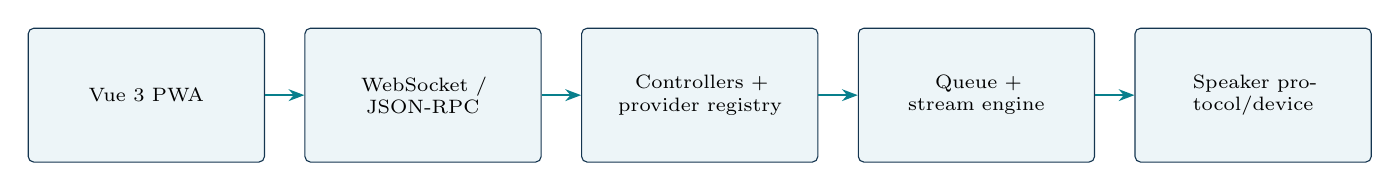
\begin{tikzpicture}[>=Stealth, node distance=1.4mm, every node/.style={font=\scriptsize,align=center}]
\node[draw=navy,rounded corners=2pt,fill=light,text width=26mm,minimum height=17mm,inner sep=2mm] (n0) {Vue 3 PWA};
\node[draw=navy,rounded corners=2pt,fill=light,text width=26mm,minimum height=17mm,inner sep=2mm,right=5mm of n0] (n1) {WebSocket / JSON-RPC};
\draw[-{Stealth[length=2mm]},thick,color=teal] (n0.east) -- (n1.west);
\node[draw=navy,rounded corners=2pt,fill=light,text width=26mm,minimum height=17mm,inner sep=2mm,right=5mm of n1] (n2) {Controllers + provider registry};
\draw[-{Stealth[length=2mm]},thick,color=teal] (n1.east) -- (n2.west);
\node[draw=navy,rounded corners=2pt,fill=light,text width=26mm,minimum height=17mm,inner sep=2mm,right=5mm of n2] (n3) {Queue + stream engine};
\draw[-{Stealth[length=2mm]},thick,color=teal] (n2.east) -- (n3.west);
\node[draw=navy,rounded corners=2pt,fill=light,text width=26mm,minimum height=17mm,inner sep=2mm,right=5mm of n3] (n4) {Speaker protocol/device};
\draw[-{Stealth[length=2mm]},thick,color=teal] (n3.east) -- (n4.west);
\end{tikzpicture}
\end{center}
\small\textit{Figure 11: Conceptual runtime path for a comparable implementation. This is not a traced source-code call graph.}\normalsize\par
\section{End-to-end user-to-speaker flow}
\begin{enumerate}[leftmargin=*,itemsep=2pt,topsep=2pt]
\item Server initializes core controllers and loads enabled provider manifests.
\item Music providers expose library/stream metadata; player providers register devices.
\item Vue frontend connects to real-time API and subscribes to state updates.
\item A play command targets queue/controller, which selects a compatible player route.
\item Stream controller prepares media and issues provider-specific device playback commands.
\item PlayerState emits normalized state back to the frontend.
\end{enumerate}
\section{Data contract [P]}
\begin{evidencebox}\small\textbf{Candidate conceptual entities (not copied database classes):}\par
\begin{itemize}[leftmargin=*,itemsep=1pt,topsep=2pt]
\item \texttt{ProviderInstance(id, domain, config\_ref)}
\item \texttt{MediaItem(provider\_id, item\_id, metadata)}
\item \texttt{Player(id, capabilities, protocol\_links)}
\item \texttt{PlayerState(public\_state, ui\_permissions)}
\item \texttt{Queue(player\_id, ordered\_entries)}
\item \texttt{StreamSession(codec, sample\_rate, target\_id)}
\end{itemize}\end{evidencebox}
\section{Implementation blueprint [P]}
\begin{itemize}[leftmargin=*,itemsep=2pt,topsep=3pt]
\item Follow the existing provider contract: manifest plus implementation, discovery, capability reporting and lifecycle hooks.
\item Keep a normalized MusicCatalog separate from provider-specific item IDs; retain source provenance.
\item Use distinct internal Player and public PlayerState models; apply permissions and transformations before serialization.
\item Centralize queue scheduling, multiroom grouping, volume control and latency compensation rules.
\item Use a bounded WebSocket event stream with reconnect/resync and HTTP endpoint for initial state.
\item Make FFmpeg/conversion paths explicit and disable unnecessary DSP/transcoding in a fidelity-first mode.
\item Ship server dependencies as a reproducible container; treat embedded service credentials as restricted resources.
\end{itemize}
\subsection*{Engineering equation}
\begin{equation*}|t_i-t_j|\le\varepsilon\quad\text{for all synchronized players }i,j\end{equation*}
A proposed multiroom playback tolerance; actual feasible epsilon depends on protocol latency, device clock and group synchronization.\par
\section{Validation and operational guardrails}
\textbf{Acceptance-test plan [P].}\par
\begin{itemize}[leftmargin=*,itemsep=2pt,topsep=3pt]
\item Provider contract tests and device discovery/unregister races.
\item State reconciliation across WebSocket reconnect and permission changes.
\item Codec/transcoding matrix for AirPlay, Chromecast and DLNA-like targets.
\item Grouped player synchronization, clock skew and buffer-underrun trials.
\end{itemize}
\textbf{Constraints and risks [B].}\par
\begin{itemize}[leftmargin=*,itemsep=2pt,topsep=3pt]
\item High integration breadth and multiple proprietary vendor APIs complicate maintenance.
\item Server relies on system FFmpeg/native utilities; bare Python install is not the documented supported distribution.
\item Apache-2.0 does not automatically license linked service credentials, API keys or non-open dependencies.
\end{itemize}
\noindent\emph{Direct repository and technical-documentation links are consolidated in the source register.}
\clearpage
\section{UI/UX architecture and annotated screen concept}
\begin{evidencebox}\small\tagverified{} Official UI documentation covers per-player queues, a persistent Player Bar, Now Playing queue/lyrics modes, audio-pipeline panel and speaker selection; the frontend uses Vue 3.\\[2pt]\textbf{UX evidence link:} \sourceurl{https://www.music-assistant.io/ui}\\[2pt]\tagproposal{} The image, colors, exact screen compositions, flows, and acceptance criteria below are authored design recommendations, not release screenshots or audited internal UI components.\end{evidencebox}
\begin{center}
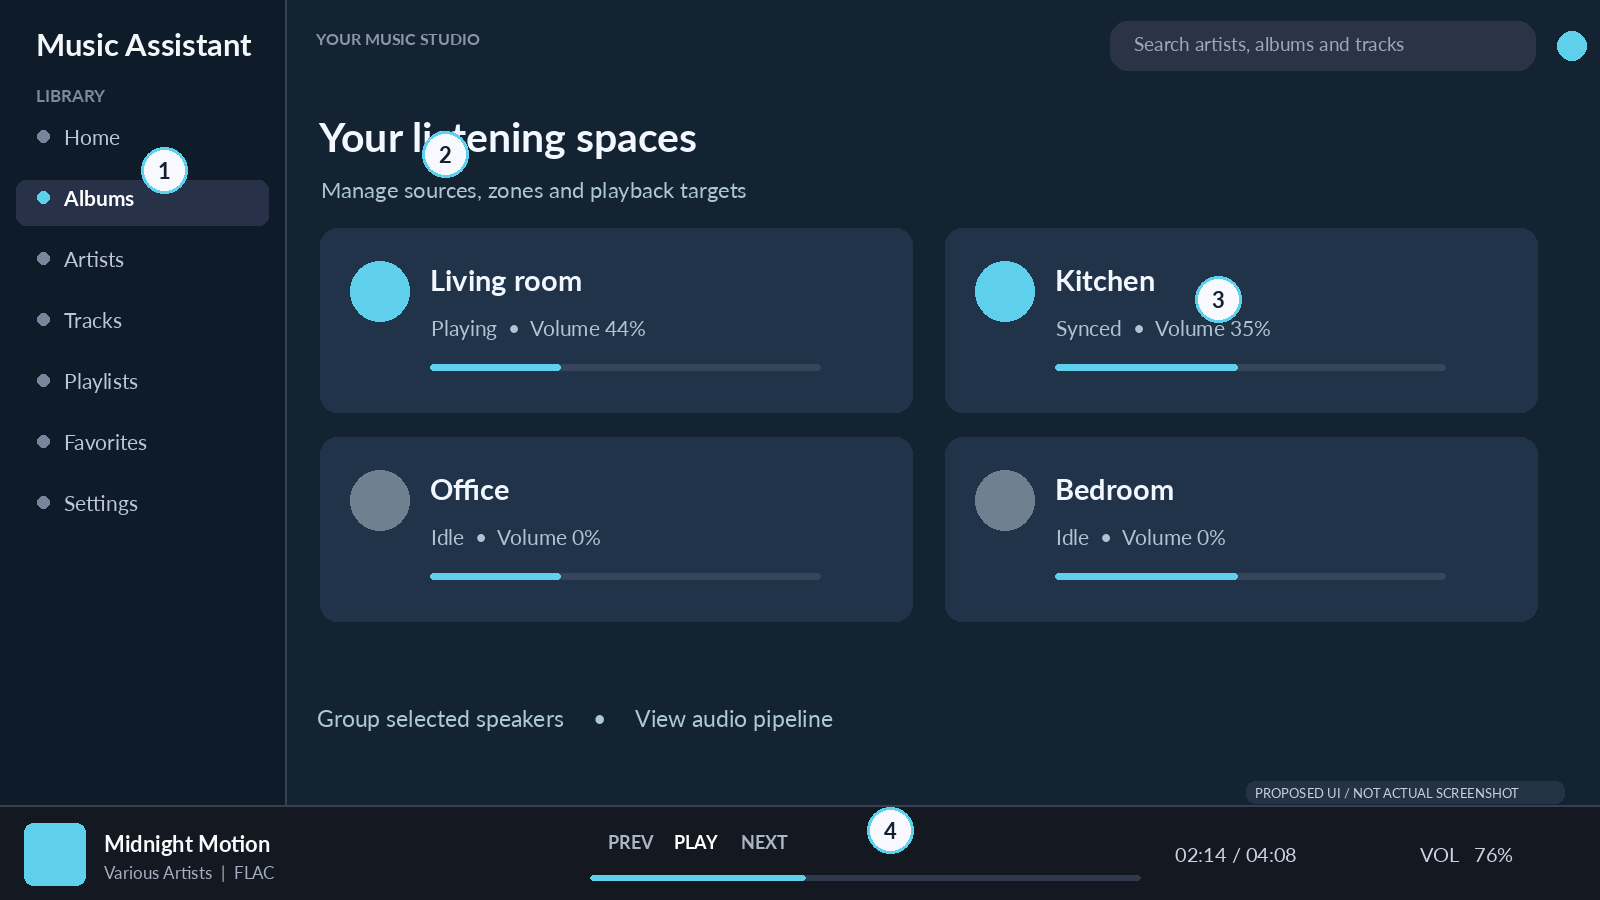
\includegraphics[width=\linewidth,height=93mm,keepaspectratio]{Music_Player_UIUX_Assets/music_assistant_concept.png}
\end{center}
{\small\color{muted}\textit{Annotated concept:} A multi-device command center rather than a single-song player. Make active target, player groups and synchronization state visible at all times. \textbf{Intended platform:} Server + Vue PWA. The visual uses invented album names and placeholder artwork.\par}
\subsection*{Proposed visual design system}
\begin{tabularx}{\linewidth}{@{}p{24mm}X@{}}
\textbf{Palette} & \colorbox[HTML]{142332}{\rule{6mm}{3mm}}\, Base 142332 \quad \colorbox[HTML]{5ED0EB}{\rule{6mm}{3mm}}\, Accent 5ED0EB \\
\textbf{Typography} & Body 14--16 px; labels 12--13 px; primary screen heading 26--34 px; numeric audio data set in tabular figures.\\
\textbf{Spacing} & 4/8 px grid; 8--16 px card radius; align cover art to text blocks; 44 px touch-target minimum where relevant.\\
\textbf{Contrast} & Target WCAG AA text contrast, 4.5:1 for normal text and 3:1 for large text; verify final palette in both light/dark states.\\
\end{tabularx}
\subsection*{Annotated interface anatomy}
\begin{tabularx}{\linewidth}{@{}p{12mm}X@{}}\toprule Mark & Proposed region and responsibilities\\\midrule
\textbf{1} & Sources and room navigation kept distinct\\
\textbf{2} & Per-room player cards and grouped device identities\\
\textbf{3} & Volume and online state communicated for each target\\
\textbf{4} & Global bar reflects the selected output and source quality\\
\bottomrule\end{tabularx}
\clearpage
\section{UX functional specification [P]}
\subsection*{Information architecture and screens}
\begin{tabularx}{\linewidth}{@{}p{34mm}X@{}}\toprule Screen / route & Core content and controls\\\midrule
Home / Sources & Music providers, library browsing, search and favorites\\
Players / Rooms & Cards for speaker targets, mute, volume and online state\\
Group \& Sync & Create/edit groups, leader, per-device latency and capabilities\\
Now Playing + Queue & Player-scoped queue, group transport, lyrics and audio pipeline\\
Provider Settings & Account state, source mappings, diagnostics and service-health view\\
\bottomrule\end{tabularx}
\subsection*{Navigation model}
Desktop left global nav + main zone grid and right inspector; compact PWA uses player selector drawer and persistent player bar.\par
\subsection*{Critical user journeys}
\begin{enumerate}[leftmargin=*,itemsep=3pt,topsep=2pt]
\item \textbf{Choose playback target.} Select a player; inspect capability badges; play song; verify active target.
\item \textbf{Group rooms.} Select compatible devices; create group; expose failures and leader assignment.
\item \textbf{Diagnose playback.} Open Now Playing; inspect pipeline; identify transcode/device; inspect recovery recommendations.
\end{enumerate}
\subsection*{Interaction, feedback and edge states}
Keyboard and touch operate volume/grouping; high-risk Remove Group action confirms consequences; real-time updates avoid focus-steal.\par
\begin{tabularx}{\linewidth}{@{}p{39mm}X@{}}\toprule State / trigger & Expected UX behavior\\\midrule
Speaker offline & Grey out target; retain historical queue; provide device diagnostic link.\\
Grouping partial failure & Show which speakers joined and which failed; permit retry/ungroup.\\
Transcoding unavoidable & Expose codec/rate and reason without suggesting bit-perfect output.\\
\bottomrule\end{tabularx}
\subsection*{Implementation and QA contract}
\begin{itemize}[leftmargin=*,itemsep=2pt,topsep=2pt]
\item \textbf{Single source of truth.} Playback, queue and current destination/device belong to the application state model, not duplicated per view.
\item \textbf{Accessibility.} Keyboard navigation, screen-reader labels, visible focus, user-controlled lyric scrolling, reduced motion and non-color-only states.
\item \textbf{Responsive behavior.} Preserve transport when resizing; test narrow, zoomed and high-font settings; use alternative to drag-only controls.
\item \textbf{Instrumentation.} speaker-selection errors; queue consistency across reconnection; sync group success; latency warnings.
\item \textbf{Boundary.} The server and frontend licenses do not automatically grant API tokens or bundled third-party integrations.
\end{itemize}
\vspace{2mm}\begin{evidencebox}\small\textbf{Prototype acceptance:} Primary play and pause remain available through every screen; the queue and playback position survive navigation; every error has recovery text; every advertised fidelity setting accurately reflects the active engine/device. Design specifications are recommendations and require product usability testing.\end{evidencebox}
\clearpage


\chapter*{Cross-product UI/UX blueprint}
\addcontentsline{toc}{chapter}{Cross-product UI/UX blueprint}
\section*{Experience principles and information architecture}
A premium experience is more than a visually rich Now Playing screen. A dependable player must make content retrieval, playback state, quality, connectivity, queue semantics and error recovery clear. The eleven concepts are \textbf{original, proposed diagrams}. They are not release screenshots or assertions that a particular product ships those precise layouts.
\begin{longtable}{@{}p{30mm}p{55mm}p{65mm}@{}}\toprule
Design layer & Shared module & Platform adaptation\\\midrule\endhead
Discovery & Search, recommendation, library filters, artist and album cards & Local apps use file/tag search; hosted clients use API/provider-specific search.\\
Playback & Transport, queue, progress, device, audio quality and lyrics & Browser media APIs, native desktop engines and Android Media3 expose different capabilities.\\
Persistence & Playlists, favorites, queue restoration, histories & File-local records and cloud accounts require different permission and conflict UX.\\
Offline & Cache, downloads, stale state and sync receipts & Only claim offline media where downloads or device files are actually present.\\
Advanced audio & Format, DSP, normalization, device and routing & Hide or disable controls unsupported by the active playback stack.\\
Multiroom & Target selection, groups, grouped queue, sync status & Relevant mainly to Music Assistant and cast-enabled integrations.\\
\bottomrule\end{longtable}
\section*{Global playback user-state model [P]}
\begin{center}
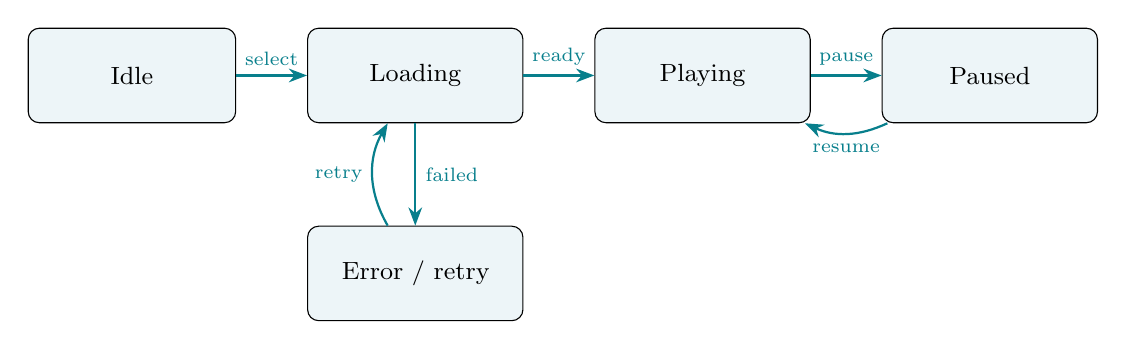
\begin{tikzpicture}[every node/.style={font=\small,align=center},>=Stealth]
\node[draw,rounded corners,fill=light,text width=24mm,minimum height=12mm] (idle) {Idle};
\node[draw,rounded corners,fill=light,text width=25mm,minimum height=12mm,right=9mm of idle] (loading) {Loading};
\node[draw,rounded corners,fill=light,text width=25mm,minimum height=12mm,right=9mm of loading] (playing) {Playing};
\node[draw,rounded corners,fill=light,text width=25mm,minimum height=12mm,right=9mm of playing] (paused) {Paused};
\node[draw,rounded corners,fill=light,text width=25mm,minimum height=12mm,below=13mm of loading] (error) {Error / retry};
\draw[-Stealth,thick,color=teal] (idle)--node[above,font=\scriptsize]{select} (loading);
\draw[-Stealth,thick,color=teal] (loading)--node[above,font=\scriptsize]{ready} (playing);
\draw[-Stealth,thick,color=teal] (playing)--node[above,font=\scriptsize]{pause} (paused);
\draw[-Stealth,thick,color=teal] (paused) to[bend left=25] node[below,font=\scriptsize]{resume} (playing);
\draw[-Stealth,thick,color=teal] (loading)--node[right,font=\scriptsize]{failed} (error);
\draw[-Stealth,thick,color=teal] (error) to[bend left=30] node[left,font=\scriptsize]{retry} (loading);
\end{tikzpicture}
\end{center}
\textbf{Contract:} All screens subscribe to one playback-state projection. Never invent progress while buffering; on error preserve the last known queue, track identity and user intent. State changes are announced to assistive technology without incessant live-region noise.
\section*{Canonical reusable UI kit [P]}
\begin{itemize}[leftmargin=*,itemsep=3pt]
\item \textbf{Primitive components:} Button, IconButton, Label, AlbumArtwork, Avatar, Input, Slider, Menu, Dialog, Toast, Skeleton, Progress, Tooltip and FocusRing.
\item \textbf{Domain components:} TrackRow, AlbumTile, MediaCard, ArtistHeader, PlaylistEditor, QualityChip, QueueList, LyricsScroller, DevicePicker, DownloadBadge and PlaybackTransport.
\item \textbf{Global shells:} Desktop side rail + content + optional inspector; mobile bottom navigation + mini-player; TV/player-dashboard variant with large remote-control targets.
\item \textbf{Tokens:} Semantic colors for foreground/surfaces/selection/error, typography scale, artwork sizes, motion timing, elevation, borders and spacing (4 px base). Generate accessible light and dark palette variants.
\item \textbf{Machine-readable states:} Every playback-relevant view consumes a discriminated union such as \texttt{idle/loading/playing/paused/buffering/error}; every loading control is cancellable where safe.
\end{itemize}
\section*{Evaluation scorecard and measurable targets [P]}
\begin{tabularx}{\linewidth}{@{}p{42mm}X@{}}\toprule
Area & Acceptance gate\\\midrule
Learnability & A first-time user reaches a playable local track or configured remote server without an unexplained dead end.\\
Playback clarity & Track title, active device, pause state and queue are reachable without destructive navigation.\\
Accessibility & Test WCAG 2.2 AA where applicable; visible keyboard focus; user-resizable text; semantic media controls and gestures with accessible equivalents.\\
Responsiveness & Verify 320/375/768/1024/1440 px layout breakpoints for web concepts; Android dynamic font and device-size classes.\\
Performance & Record first-action response, scan feedback, seek lag, artwork load and route-switch frame drops on budget devices.\\
Fidelity honesty & The displayed codec/quality indicator refers to the current asset or output path and never asserts hardware bit-perfect operation without tests.\\
Reliability & Test device removal, permission denial, network loss, queue restoration, audio focus interruption, resume and download corruption.\\
\bottomrule\end{tabularx}
\section*{Recommended product handoff deliverables}
For development, create a real design file with the eleven reference concepts as separate pages; define semantic tokens, inspectable component variants, default/hover/focus/disabled/loading/error states, breakpoint frames, motion guidelines, localization behavior and executable interaction prototypes. Document route-to-API dependency for every screen and maintain screenshot regression tests before rebuilding interfaces in another framework.
\clearpage
\chapter*{Cross-project product blueprint}
\addcontentsline{toc}{chapter}{Cross-project product blueprint}
\section*{Reference architecture if building a new premium player}
For a product that must combine the visual polish of Feishin/Koel with offline and Hi-Fi behavior, use a modular design with explicit platform and fidelity capability boundaries. The diagram below is a \emph{proposed new architecture}, not a description of any single repository.
\begin{center}
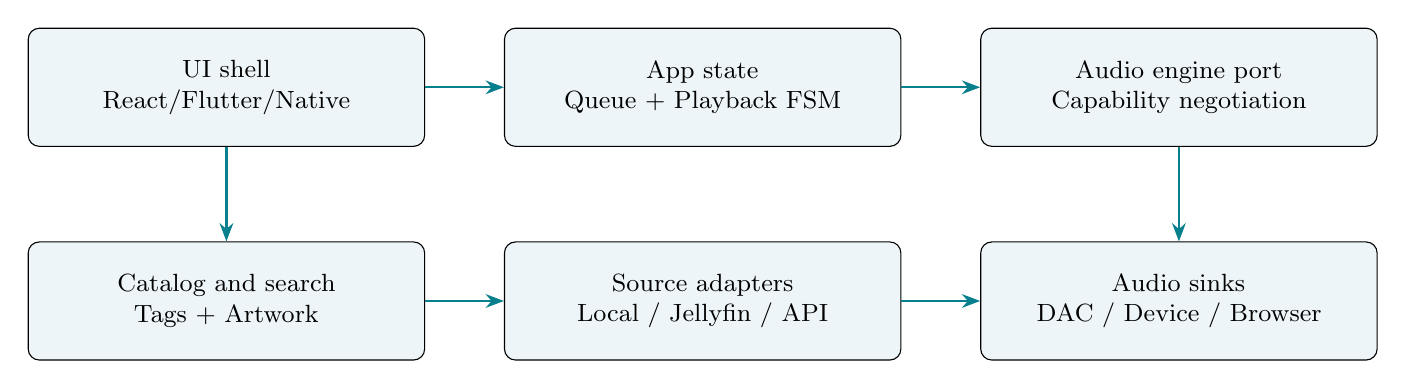
\begin{tikzpicture}[node distance=5mm, every node/.style={font=\small,align=center},>=Stealth]
\node[draw,rounded corners,fill=light,text width=48mm,minimum height=15mm] (ui) {UI shell\\React/Flutter/Native};
\node[draw,rounded corners,fill=light,text width=48mm,minimum height=15mm,right=10mm of ui] (state) {App state\\Queue + Playback FSM};
\node[draw,rounded corners,fill=light,text width=48mm,minimum height=15mm,right=10mm of state] (audio) {Audio engine port\\Capability negotiation};
\node[draw,rounded corners,fill=light,text width=48mm,minimum height=15mm,below=12mm of ui] (catalog) {Catalog and search\\Tags + Artwork};
\node[draw,rounded corners,fill=light,text width=48mm,minimum height=15mm,right=10mm of catalog] (source) {Source adapters\\Local / Jellyfin / API};
\node[draw,rounded corners,fill=light,text width=48mm,minimum height=15mm,right=10mm of source] (sink) {Audio sinks\\DAC / Device / Browser};
\draw[-Stealth,thick,color=teal] (ui)--(state);
\draw[-Stealth,thick,color=teal] (state)--(audio);
\draw[-Stealth,thick,color=teal] (ui)--(catalog);
\draw[-Stealth,thick,color=teal] (catalog)--(source);
\draw[-Stealth,thick,color=teal] (source)--(sink);
\draw[-Stealth,thick,color=teal] (audio)--(sink);
\end{tikzpicture}
\end{center}
\section*{Shared domain interfaces [P]}
\begin{itemize}[leftmargin=*]
\item \texttt{CatalogProvider}: scan/search/getTrack/getAlbum/getArtwork and supported capabilities.
\item \texttt{StreamResolver}: choose local file, authorized direct stream or declared transcode output.
\item \texttt{PlaybackEngine}: load/play/pause/seek/device/volume with explicit state and errors.
\item \texttt{QueueStore}: insert, remove, reorder, shuffle, repeat, persistence and crash restoration.
\item \texttt{PlaybackPolicy}: optional DSP, normalization, loudness, crossfade, replay gain, fidelity mode.
\item \texttt{DeviceRegistry}: supported codec, sample rate, bit depth, exclusive-output and latency information.
\end{itemize}
\section*{A sensible delivery sequence [P]}
\begin{enumerate}[leftmargin=*]
\item \textbf{Foundation.} Decide browser, desktop, Android or server-first deployment; establish license boundary and architecture decision records.
\item \textbf{Core playback.} Implement queue FSM, local file playback, seek, media controls, error recovery and a reproducible audio test harness.
\item \textbf{Library.} Tag extraction, incremental indexing, album art, search, playlists and migration versioning.
\item \textbf{Polish.} Design tokens, artwork animation, typography, theme variants, keyboard/assistive access and performance budgets.
\item \textbf{Advanced listening.} Gapless, ReplayGain, device negotiation, sample-rate display, optional DSP and playback-path diagnostics.
\item \textbf{Connected audio.} Add remote servers, cache/offline, multi-user, scrobble and casting as separately testable adapters.
\end{enumerate}
\section*{Fidelity measurement boundaries}
\begin{align*}
T_{\mathrm{startup}} &= t_{\mathrm{first\ audible\ sample}}-t_{\mathrm{play\ command}},\\
\mathrm{BufferHeadroom} &= \frac{N_{\mathrm{available\ frames}}}{f_s},\\
\mathrm{Underruns/min} &= \frac{60\,N_{\mathrm{underruns}}}{T_{\mathrm{played\ seconds}}}.
\end{align*}
Collect these alongside crash-free sessions, scan/index lag, memory use, network rebuffering and gapless edge silence. Only describe a playback path as bit-perfect when decoded samples, processing configuration, OS audio path and device behavior have been tested for the exact target platform.

\section*{Final decision notes}
\begin{longtable}{@{}p{33mm}p{47mm}p{58mm}@{}}\toprule
Objective & Examine first & Reason / caveat\\\midrule\endhead
Premium client for owned server & Feishin & Highly polished; relies on separate server; GPL.\\
Custom web streaming platform & Koel & Strong Laravel/Vue core; MIT, Plus separated.\\
Elegant local desktop & Museeks; Tauon & MIT lightweight base versus GPL native playback.\\
Audiophile output & Strawberry & Rich Hi-Fi claims; Qt and GPL.\\
Offline mobile & Finamp & Flutter + Jellyfin + offline; MPL.\\
Native Android UI & Gramophone; Auxio; Retro & Media3/metadata/theming emphasis; GPL.\\
Self-hosted personalization & Swing Music & Python server; AGPL + premium distinction.\\
Whole-home speaker control & Music Assistant & Providers, streams, groups; Apache-2.0 with dependency caveats.\\
\bottomrule\end{longtable}

\chapter*{Source register and confidence statement}
\addcontentsline{toc}{chapter}{Source register and confidence statement}
\textbf{All source URLs are clickable in the individual project chapters.} The report uses first-party GitHub README files, observable repository-root structures, build manifests, technical docs and project licensing notices. In particular: Tauon's current native extension is established by \href{https://github.com/Taiko2k/Tauon/blob/master/pyproject.toml}{pyproject.toml} and GStreamer removal is established by its \href{https://github.com/Taiko2k/Tauon/blob/master/CHANGELOG.md}{changelog}; Music Assistant's provider, webserver and player-controller interfaces are documented in the linked \texttt{DEVELOPMENT.md} and controller READMEs; Swing Music's premium native-module packaging is visible in its \href{https://github.com/swingmx/swingmusic/blob/master/Dockerfile}{Dockerfile}.

\textbf{Verification level:} Repository/readme/documentation inspection, not compilation, runtime probing, code-complete reverse engineering or security audit. The [P] architecture diagrams, conceptual UI mockups, screen inventories, interaction models, data fields, contracts, equations and plans are intentionally authored blueprint artifacts, and their presence is not evidence that a project implements them identically. Re-run a license and source revision review immediately before reusing code.
\section*{Complete first-party repository index}
\begin{longtable}{@{}p{38mm}p{112mm}@{}}\toprule Project & Canonical repository and inspected documentation\\\midrule\endhead
Feishin & \href{https://github.com/jeffvli/feishin}{GitHub source} $\cdot$ \href{https://github.com/jeffvli/feishin/blob/development/README.md}{Additional source}\\
Tauon & \href{https://github.com/Taiko2k/Tauon}{GitHub source} $\cdot$ \href{https://github.com/Taiko2k/Tauon/blob/master/pyproject.toml}{Additional source} $\cdot$ \href{https://github.com/Taiko2k/Tauon/blob/master/CHANGELOG.md}{Additional source}\\
Koel & \href{https://github.com/koel/koel}{GitHub source} $\cdot$ \href{https://docs.koel.dev/}{Project docs} $\cdot$ \href{https://github.com/koel/koel/blob/master/README.md}{Additional source}\\
Swing Music & \href{https://github.com/swingmx/swingmusic}{GitHub source} $\cdot$ \href{https://github.com/swingmx/swingmusic/blob/master/Dockerfile}{Additional source} $\cdot$ \href{https://github.com/swingmx/webclient}{Additional source}\\
Museeks & \href{https://github.com/martpie/museeks}{GitHub source} $\cdot$ \href{https://github.com/martpie/museeks/blob/master/README.md}{Additional source}\\
Strawberry & \href{https://github.com/strawberrymusicplayer/strawberry}{GitHub source} $\cdot$ \href{https://github.com/strawberrymusicplayer/strawberry/blob/master/README.md}{Additional source}\\
Finamp & \href{https://github.com/finamp-app/finamp}{GitHub source} $\cdot$ \href{https://github.com/finamp-app/finamp/blob/redesign/README.md}{Additional source}\\
Gramophone & \href{https://github.com/FoedusProgramme/Gramophone}{GitHub source} $\cdot$ \href{https://github.com/FoedusProgramme/Gramophone/blob/beta/readme.md}{Additional source}\\
Auxio & \href{https://github.com/OxygenCobalt/Auxio}{GitHub source} $\cdot$ \href{https://github.com/OxygenCobalt/Auxio/blob/dev/README.md}{Additional source}\\
Retro Music Player & \href{https://github.com/RetroMusicPlayer/RetroMusicPlayer}{GitHub source} $\cdot$ \href{https://retromusic.app/RetroMusicPlayer}{Additional source} $\cdot$ \href{https://github.com/RetroMusicPlayer/RetroMusicPlayer/blob/dev/README.md}{Additional source}\\
Music Assistant & \href{https://github.com/music-assistant/server}{GitHub source} $\cdot$ \href{https://github.com/music-assistant/frontend}{Additional source} $\cdot$ \href{https://github.com/music-assistant/server/blob/dev/DEVELOPMENT.md}{Technical docs} $\cdot$ \href{https://github.com/music-assistant/server/blob/dev/music_assistant/controllers/players/README.md}{Technical docs} $\cdot$ \href{https://github.com/music-assistant/server/blob/dev/music_assistant/controllers/webserver/README.md}{Technical docs}\\
\bottomrule\end{longtable}
\end{document}
